\documentclass[12pt,a4paper]{article}
\usepackage[brazil]{babel}
\usepackage[T1]{fontenc}
\usepackage[utf8]{inputenc}
\usepackage[tmargin=2cm, bmargin=2cm, lmargin=2cm, rmargin=2cm]{geometry}
\usepackage{float}
\usepackage{indentfirst}
\usepackage{graphicx}
\usepackage{listings}
\usepackage{pdfpages}
\lstset{language=XML,basicstyle=\ttfamily,breaklines=true}
\usepackage[pdftex]{hyperref}
\hypersetup{
    colorlinks=true,
    linkcolor=cyan,
    filecolor=magenta,      
    urlcolor=blue,
}

\urlstyle{same}

\title{Comparação de Desempenho de servidores MQTT}
\author{Bruno Carneiro da Cunha \\ \href{mailto:brunocarneirodacunha@usp.br}{<brunocarneirodacunha@usp.br>}}

\begin{document}
\maketitle
    
\section{Introdução}
Nos últimos anos, aplicativos baseados em MQTT aumentaram bastante fazendo com que esse seja o protocolo pub/sub mais popular do mundo, com utilização em uma ampla variedade de domínios como saúde, automação residencial, transportes inteligentes e distribuição de energia. Apesar da popularidade, faltam soluções que garantam uma boa segurança do MQTT. De fato, o protocolo não foi desenvolvido com segurança em mente.

A fim de realizar experimentos para avaliar a segurança do MQTT, o mesmo deverá ser implantado em duas redes de experimentação que serão construídas na USP e na UNIFESP. O protocolo será integrado em uma plataforma para cidades inteligentes chamada \href{https://interscity.org/}{InterSCity}, que foi desenvolvida dentro do escopo do projeto de mesmo nome.

Este relatório apresenta uma comparação de performance entre três implementações de servidores, ou \textit{brokers}, MQTT. Através dos testes e dos seus resultados, pretende-se justificar a escolha de uma implementação para a integração à plataforma.

\section{Ambiente de Experimentação}

Cada teste foi executado em três ambientes de rede diferentes. No primeiro, os clientes MQTT e o servidor se comunicaram através da interface virtual de loopback de uma máquina com dois cores \textit{Intel i5} de 1,6 GHz.

No segundo, os clientes executaram na mesma máquina, porém comunicaram-se através de uma rede Wi-Fi 2,4 GHz residencial com um \textit{broker} que se encontrava em um computador de quatro cores \textit{Intel i7} de 2,2 GHz. Ambos os computadores possuem interfaces de rede Wi-Fi do fabricante Broadcom, modelo BCM43xx 1.0. Também havia tráfego de outros computadores nessa rede.
\begin{center}
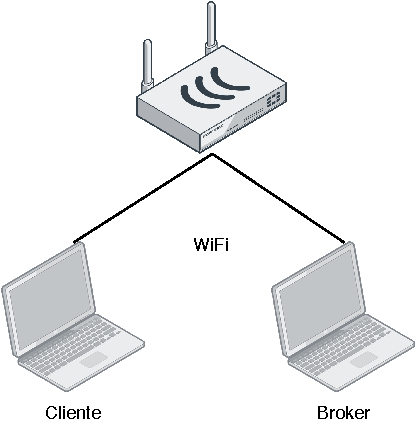
\includegraphics[width=0.5\textwidth]{wifi}
\end{center}

No terceiro ambiente, conectou-se as duas máquinas mencionadas acima através de uma rede Ethernet direta, sem intermediário. Os clientes e broker rodaram em seus respectivos \textit{hosts}. As duas máquinas possuem interfaces Ethernet 10/100/1000.
\begin{center}
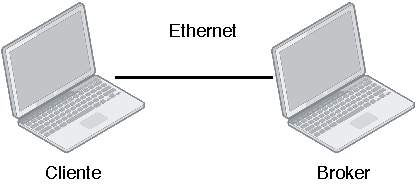
\includegraphics[width=0.5\textwidth]{ethernet}
\end{center}

O computador de dois cores executou os seus programas no sistema operacional macOS 10.14.4, e o computador de quatro cores executou no sistema macOS 10.13.6. Os clientes de teste rodaram o script \href{https://github.com/batmacumba/mqttperf}{mqttperf}, escrito em Ruby, usando a implementação de cliente MQTT do projeto  \href{https://github.com/eclipse/paho.mqtt.ruby}{Eclipse Paho}.


\section{Implementações de Brokers Testadas}
Dadas as necessidades do projeto somente era interessante testar as implementações de código aberto, e que possuíam capacidade de servir clientes através de conexões seguras TLS/SSL. Por isso, de uma lista extensa de implementações, somente as seguintes foram consideradas:

\begin{center}
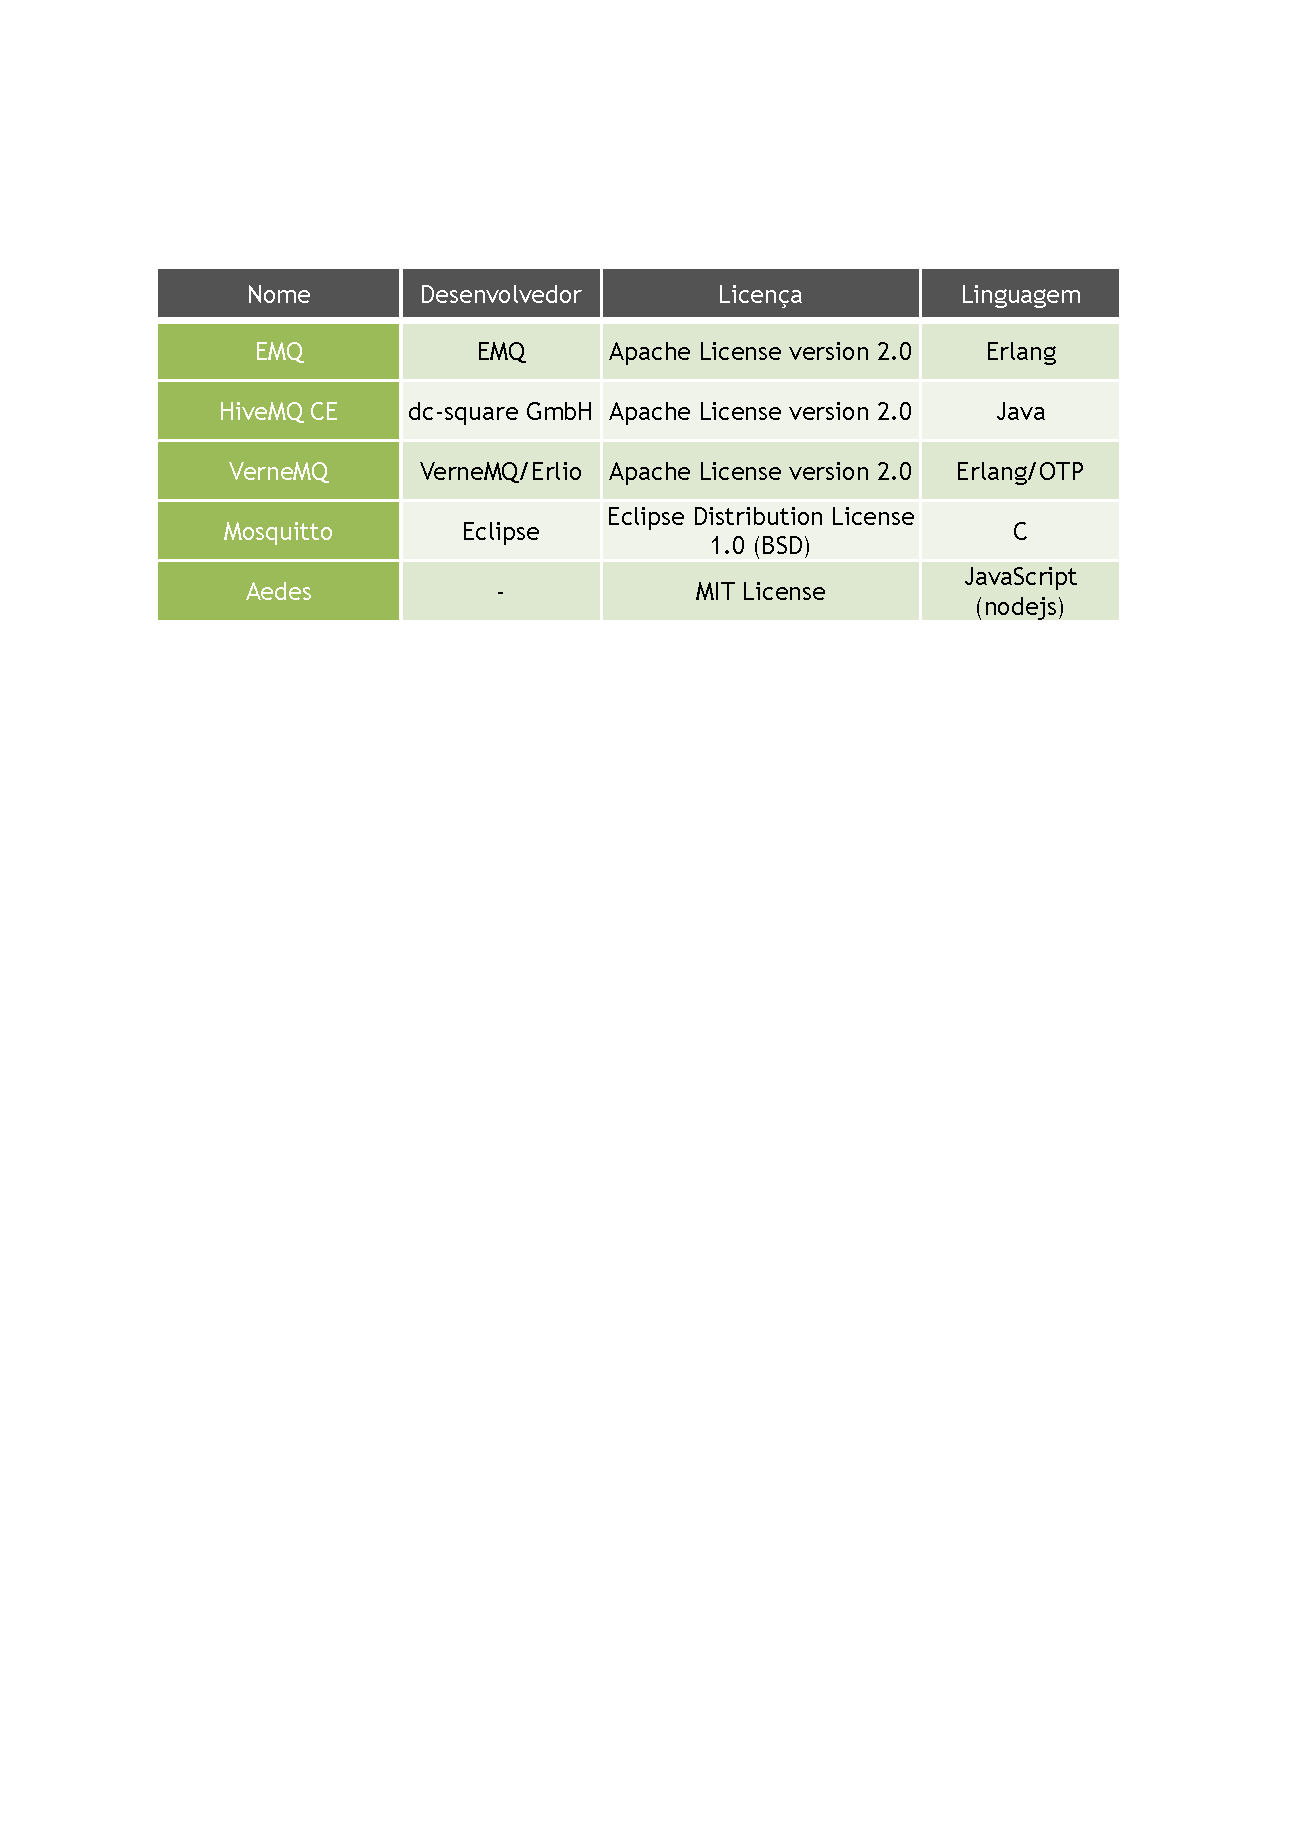
\includegraphics[width=0.9\textwidth]{brokers}
\end{center}

Das escolhas acima, não foi possível instalar o broker EMQ, pois o link de download do binário no site oficial estava quebrado. E também não foi possível testar o servidor VerneMQ, pois o broker resetava a conexão TCP assim que qualquer cliente tentava conectar-se à sua porta.

Logo, as implementações testadas foram Mosquitto v1.6.9, Aedes v0.41.0 e HiveMQ v1.10.

\section{Experimentos Planejados}

O protocolo MQTT prevê as seguintes mensagens:
\begin{center}
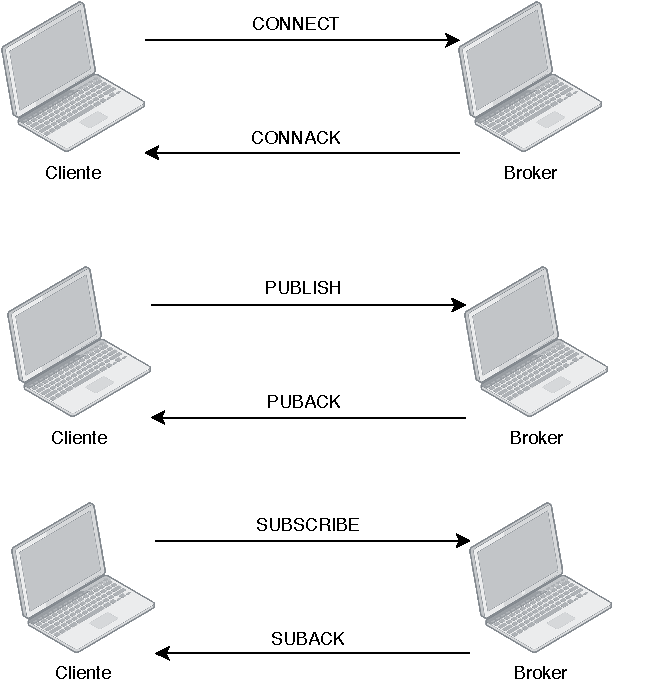
\includegraphics[width=0.7\textwidth]{mqtt}
\end{center}

Na mensagem CONNECT, o cliente tenta se conectar ao broker, informando a versão do protocolo, um identificador e configurando algumas flags, enquanto o servidor responde com CONNACK, aceitando ou não a conexão.

Na mensagem PUBLISH o cliente publica uma mensagem em algum tópico, o servidor responde com PUBACK. A mensagem do tipo PUBLISH também é transmitida pelo broker aos assinantes de um determinado tópico, quando houver uma mensagem nova.

Na mensagem SUBSCRIBE, um cliente requisita assinar um tópico, ou seja, informa ao servidor que deseja receber todas as novas mensagens publicadas naquele tópico. O servidor responde com SUBACK se a requisição for aceita.

Planejou-se testar a performance dos brokers através do teste de escrita, de leitura e de difusão das mensagens, de acordo com os diagramas a seguir:

\begin{center}
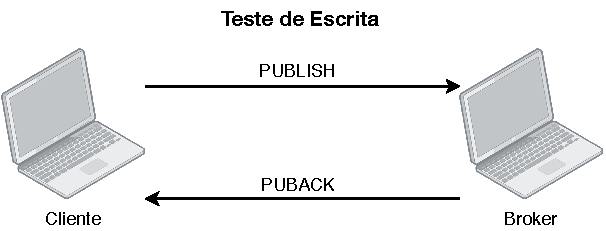
\includegraphics[width=0.7\textwidth]{write}
\end{center}
\begin{center}
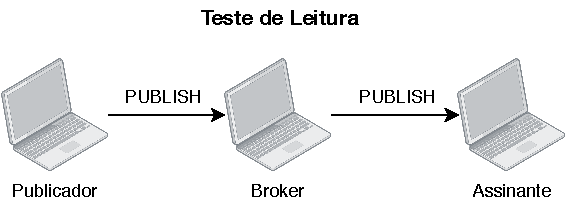
\includegraphics[width=0.7\textwidth]{read}
\end{center}

No teste de escrita, conta-se o intervalo de tempo entre o envio da mensagem PUBLISH, e o recebimento de PUBACK. Repetiu-se o teste 1000 vezes, calculando-se a média e o desvio padrão das amostras. O teste de leitura consiste do mesmo procedimento, mas conta-se o intervalo de tempo entre o envio da mensagem PUBLISH, e o recebimento da mesma pelo único cliente assinante do tópico. Ambos os conjuntos de testes foram feitos com mensagens comprimento de 1 byte, e com mensagens de comprimento de 1000 bytes.

\begin{center}
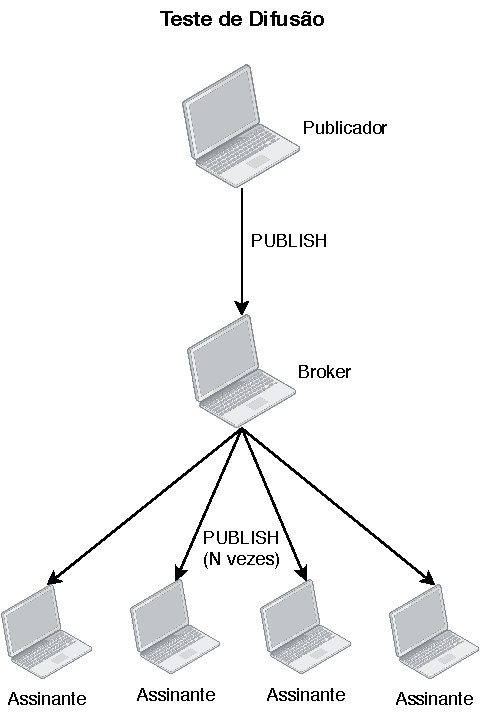
\includegraphics[width=0.6\textwidth]{spread}
\end{center}

O teste de difusão consiste em contar o intervalo de tempo entre o envio de PUBLISH pelo cliente publicador, e o recebimento da mensagem por cada assinante daquele tópico. Calcula-se a média entre os intervalos contados por cada assinante. Esse teste foi repetido 20 vezes, calculando-se o desvio padrão entre as médias resultantes. O teste foi executado com mensagens de comprimento 1 byte, em tópicos com $N$ assinantes, sendo $N = [10, 50, 100, 200]$.

Todos os testes de escrita, leitura e difusão foram rodados em duas modalidades: conexão insegura \textit{plaintext}, e conexão criptografada através de TLS/SSL.

Novamente, o script usado para rodar os testes encontra-se no repositório \href{https://github.com/batmacumba/mqttperf}{mqttperf}, e os dados brutos dos testes podem ser encontrados \href{https://github.com/batmacumba/mqtt}{aqui}.

\section{Resultados Encontrados}

\subsection{Fluxo de Dados}
Os dados brutos gerados pelo script \textit{mqttperf} foram individualmente guardados em arquivos de texto. Os resultados dos testes de escrita e leitura foram manualmente digitados na tabela de dados que gerou os gráficos abaixo. Os resultados dos testes de difusão foram extraídos através de scripts em \textit{Python} e processados para achar os valores de média e desvio padrão. Esses valores então foram manualmente digitados. Todos os gráficos foram gerados através de tabelas criadas no programa \textit{Numbers}. Todos os scripts estão disponíveis no \href{https://github.com/batmacumba/mqtt}{repositório}.

\subsection{Localhost}
\subsubsection{Escrita/Leitura}
\begin{center}
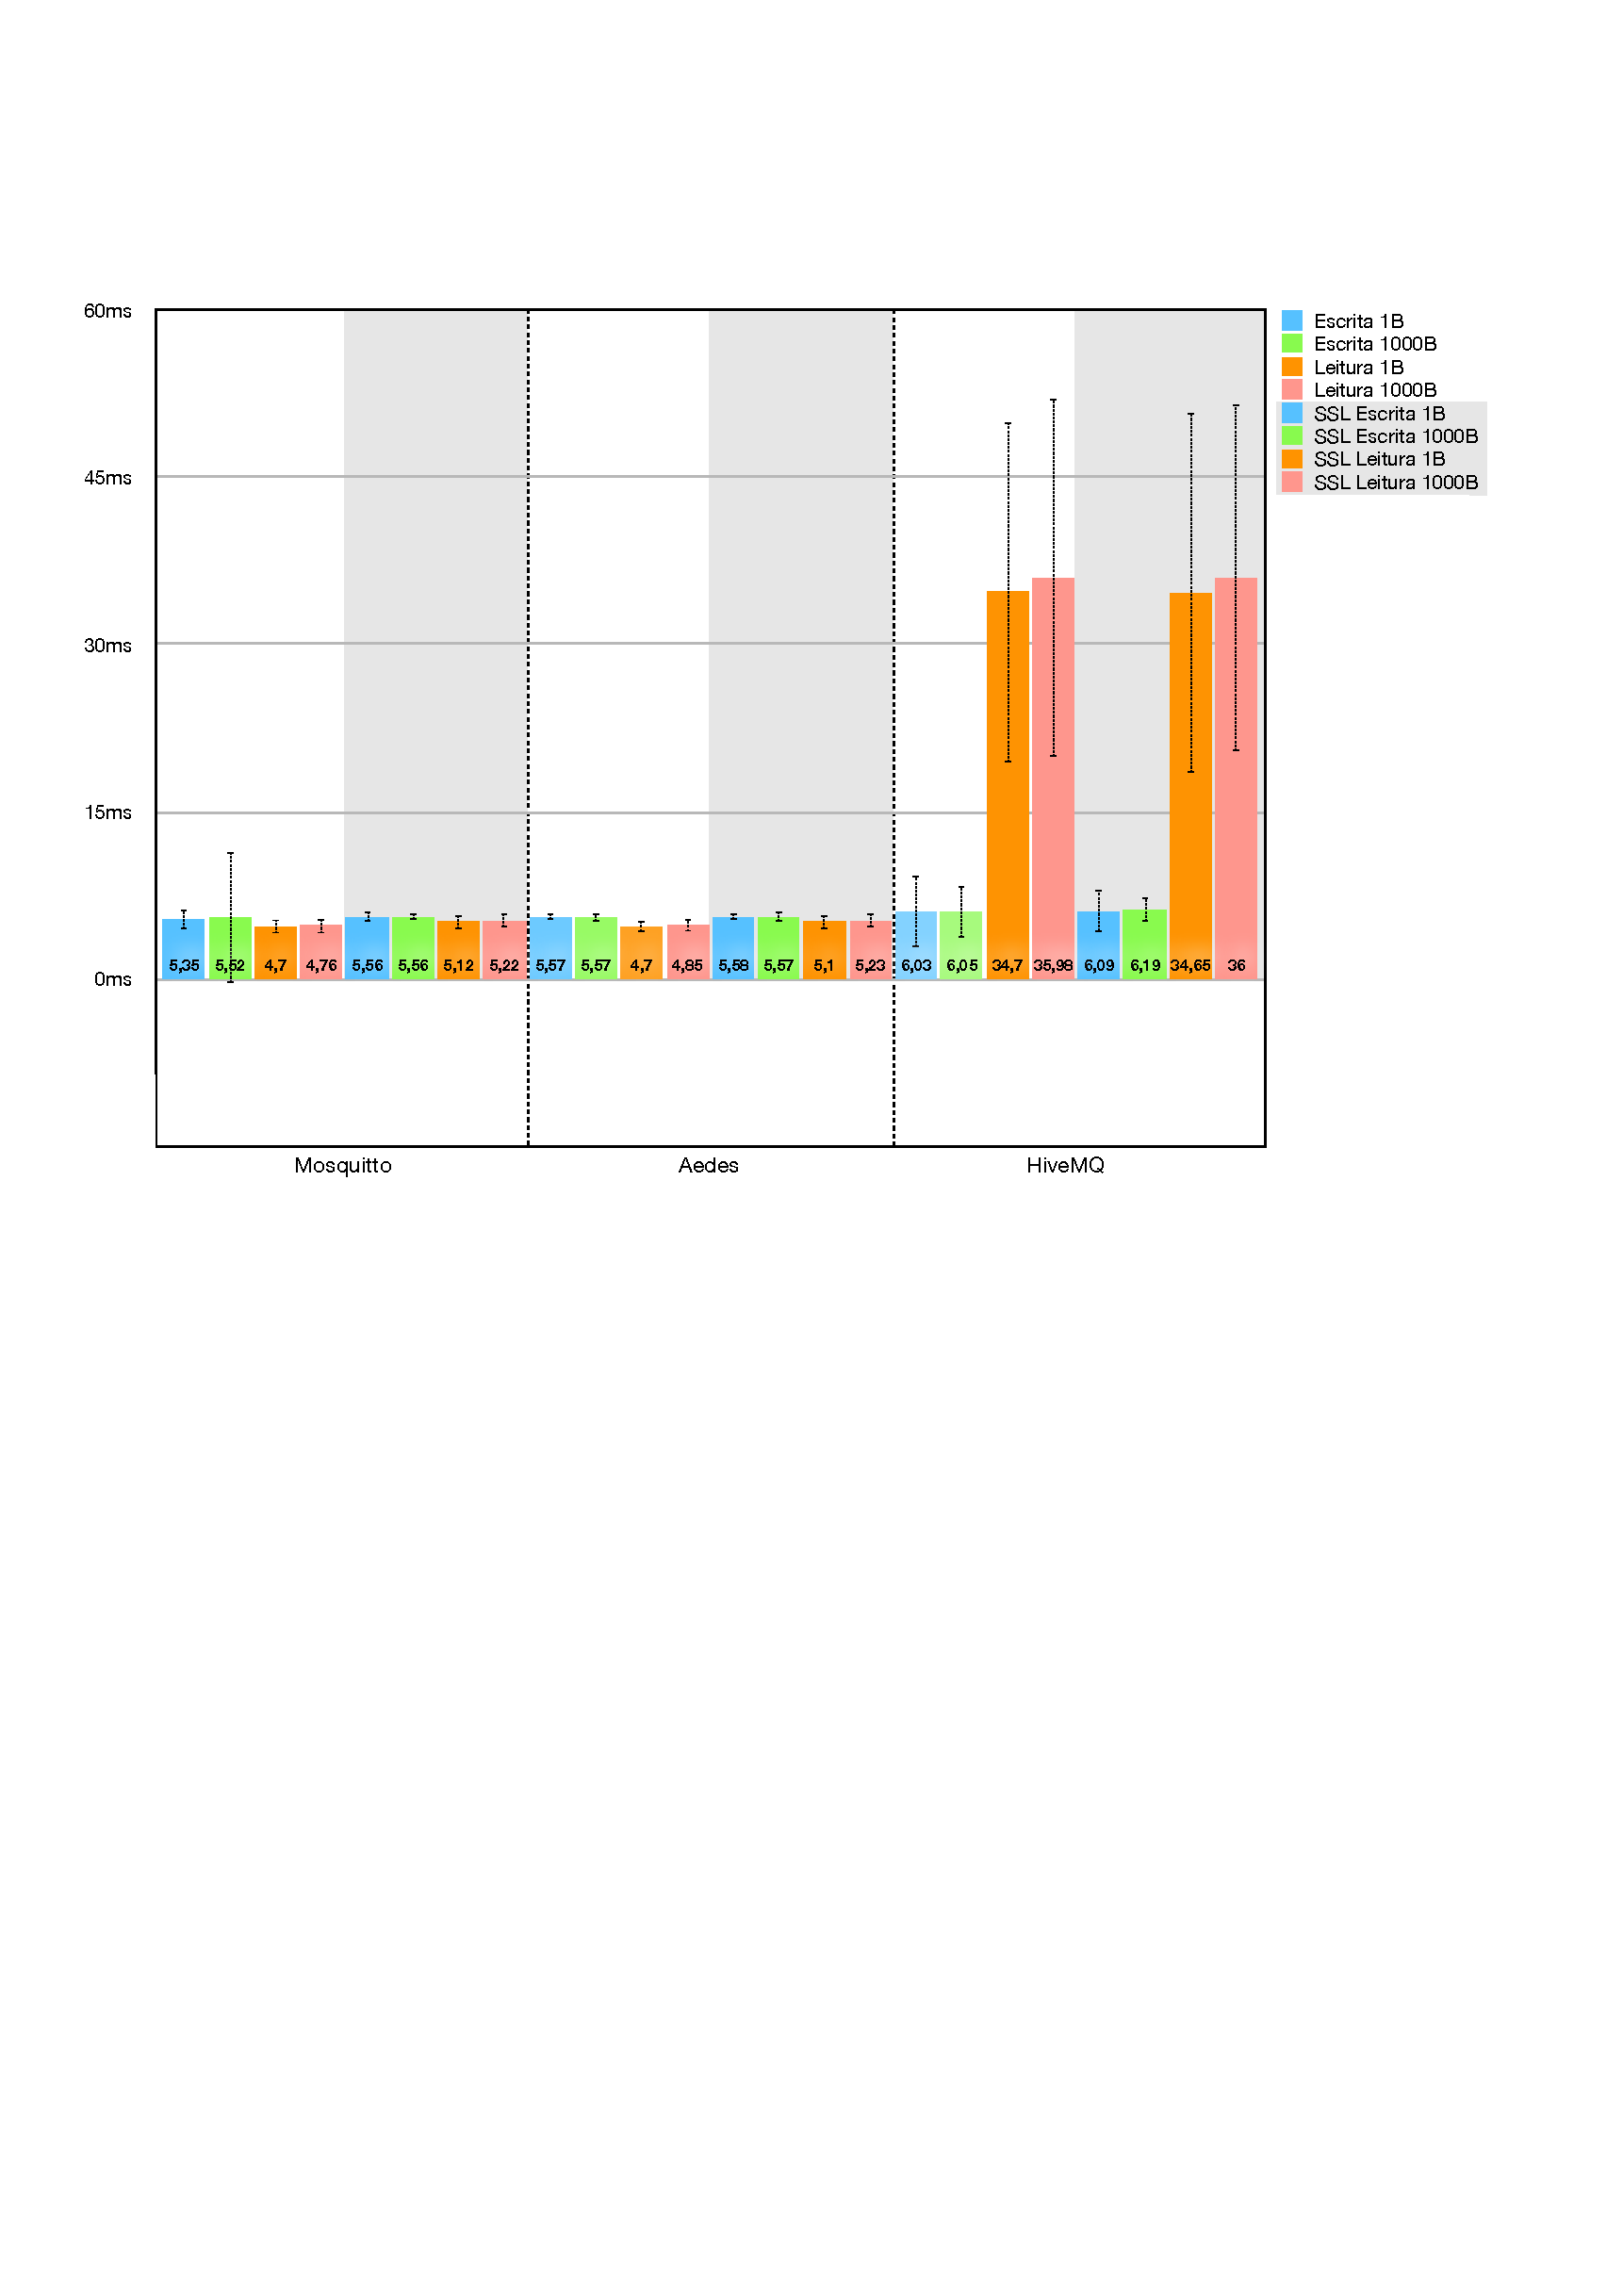
\includegraphics[width=1.0\textwidth]{local_wr.pdf}
\end{center}
\subsubsection{Difusão N = [10, 50, 100]}
\begin{center}
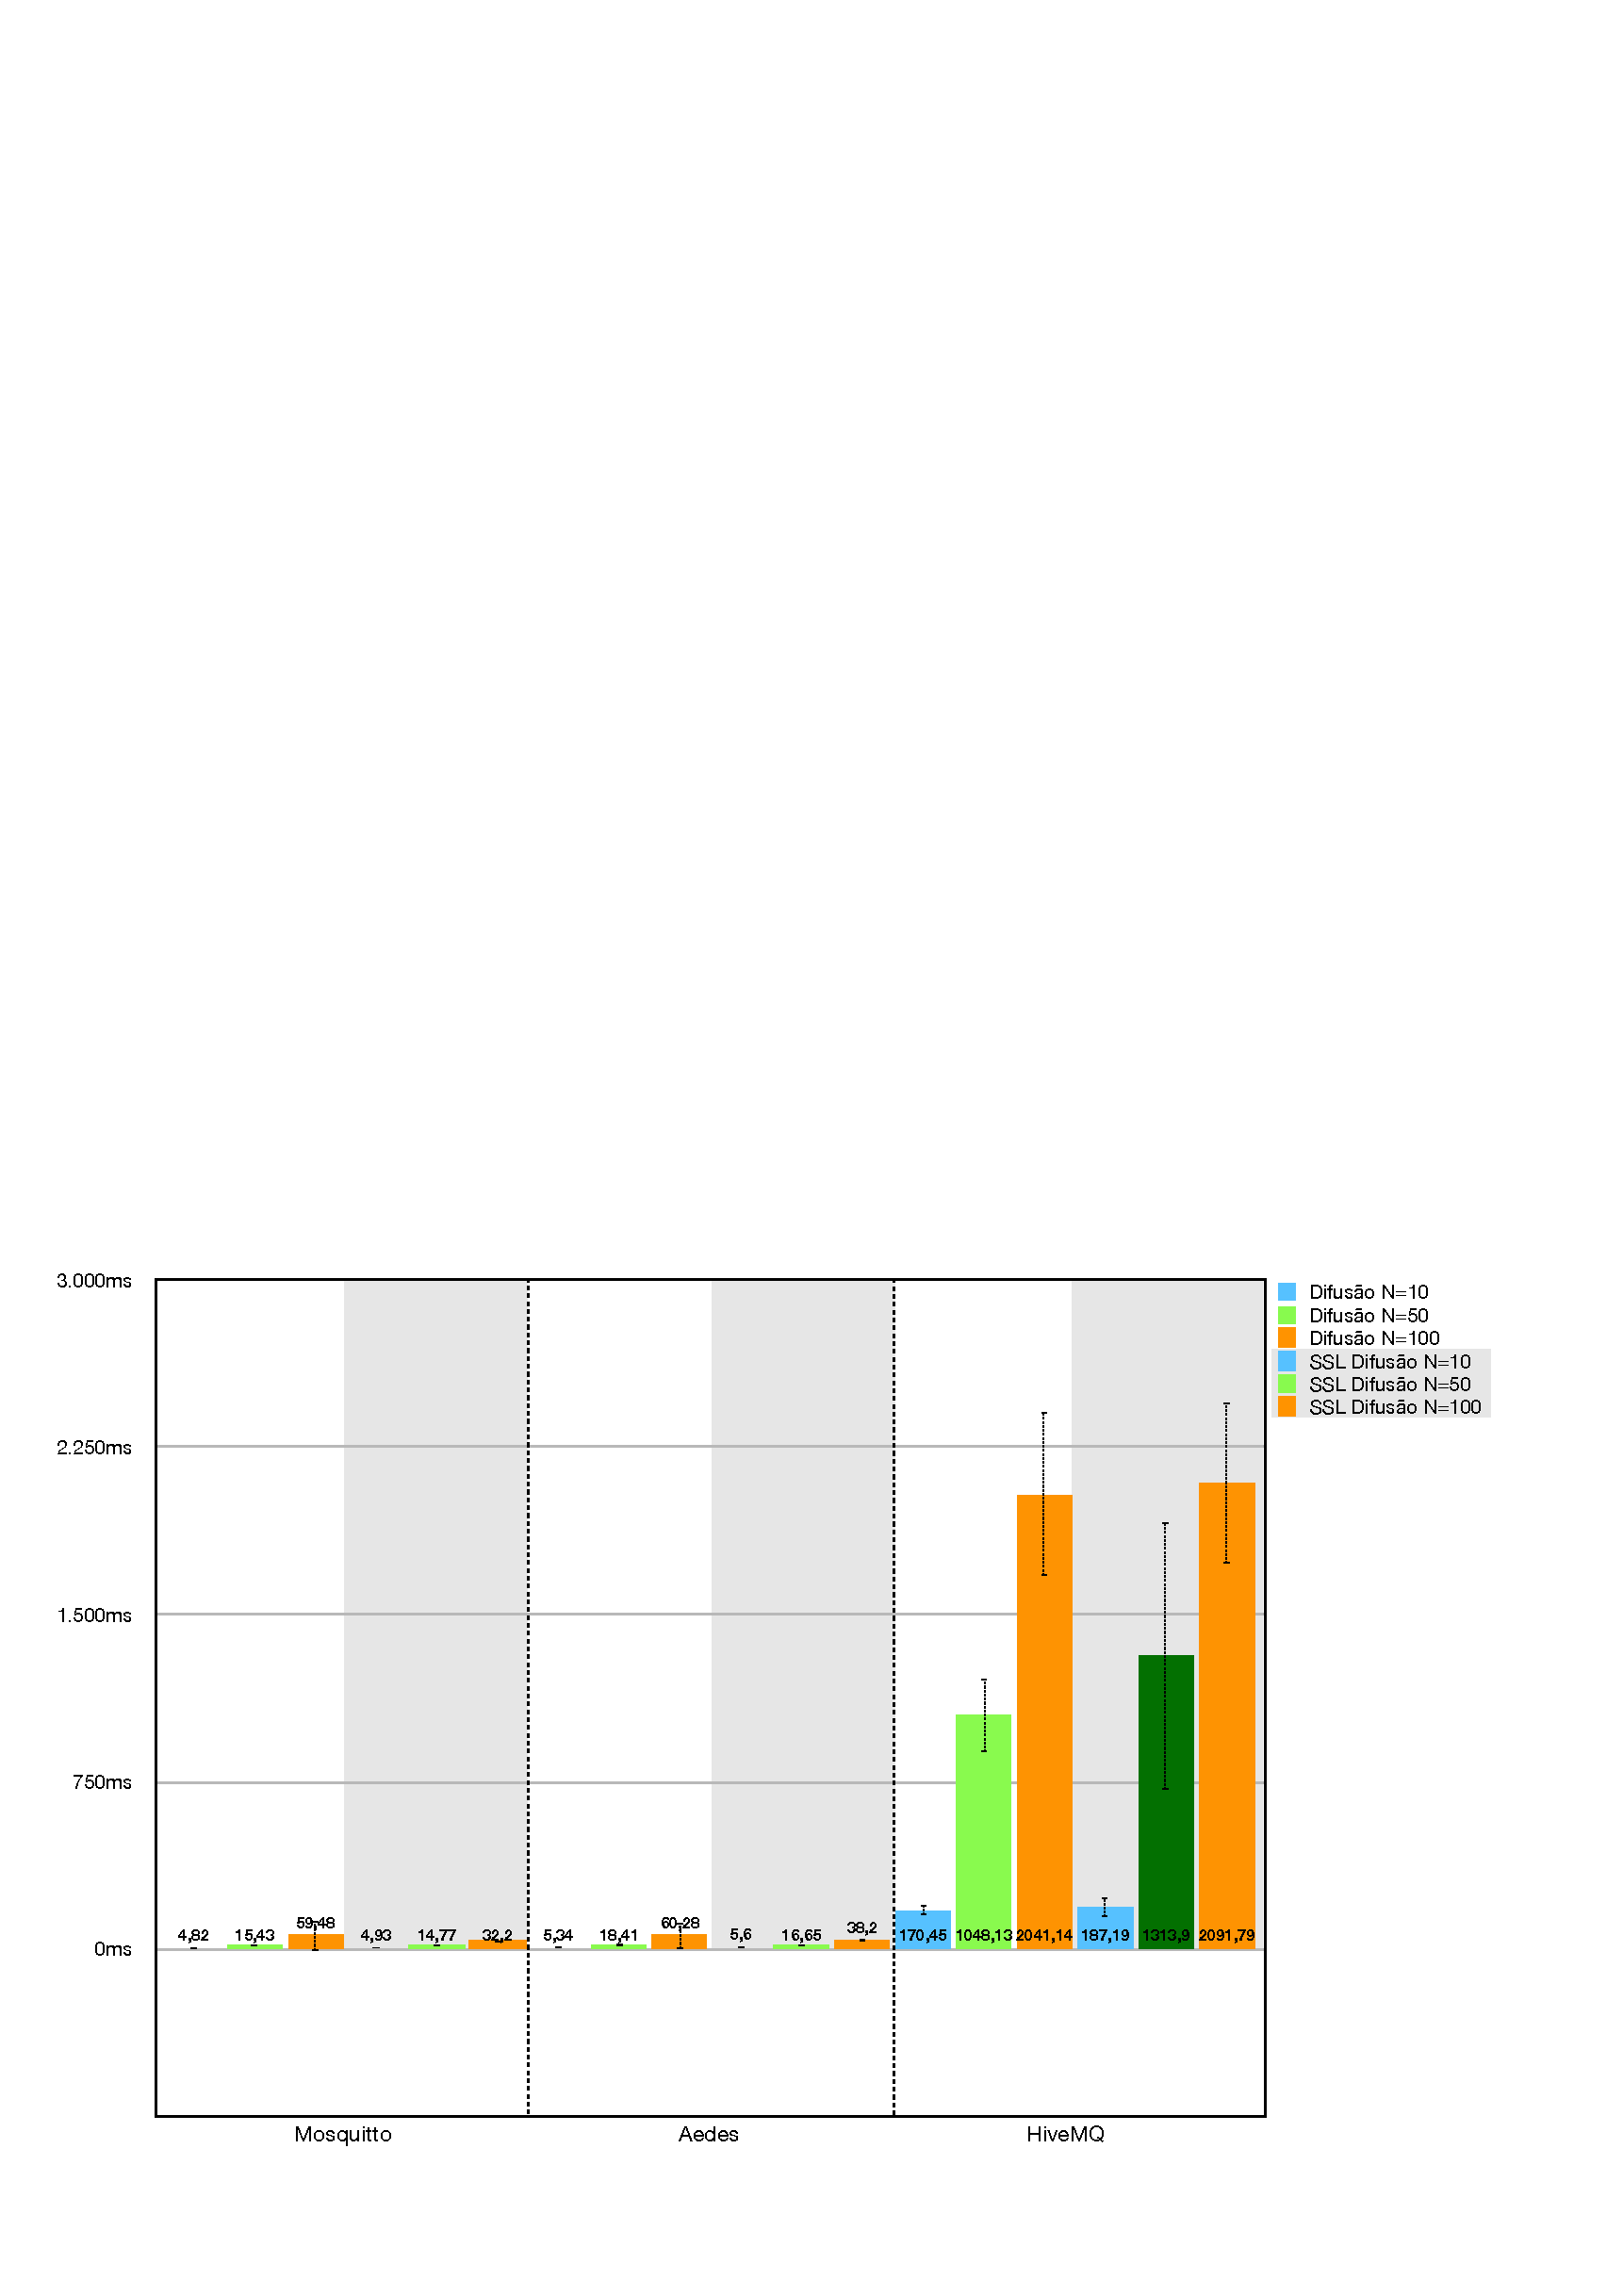
\includegraphics[width=1.0\textwidth]{local_spread1.pdf}
\end{center}
\subsubsection{Difusão N = 200}
\begin{center}
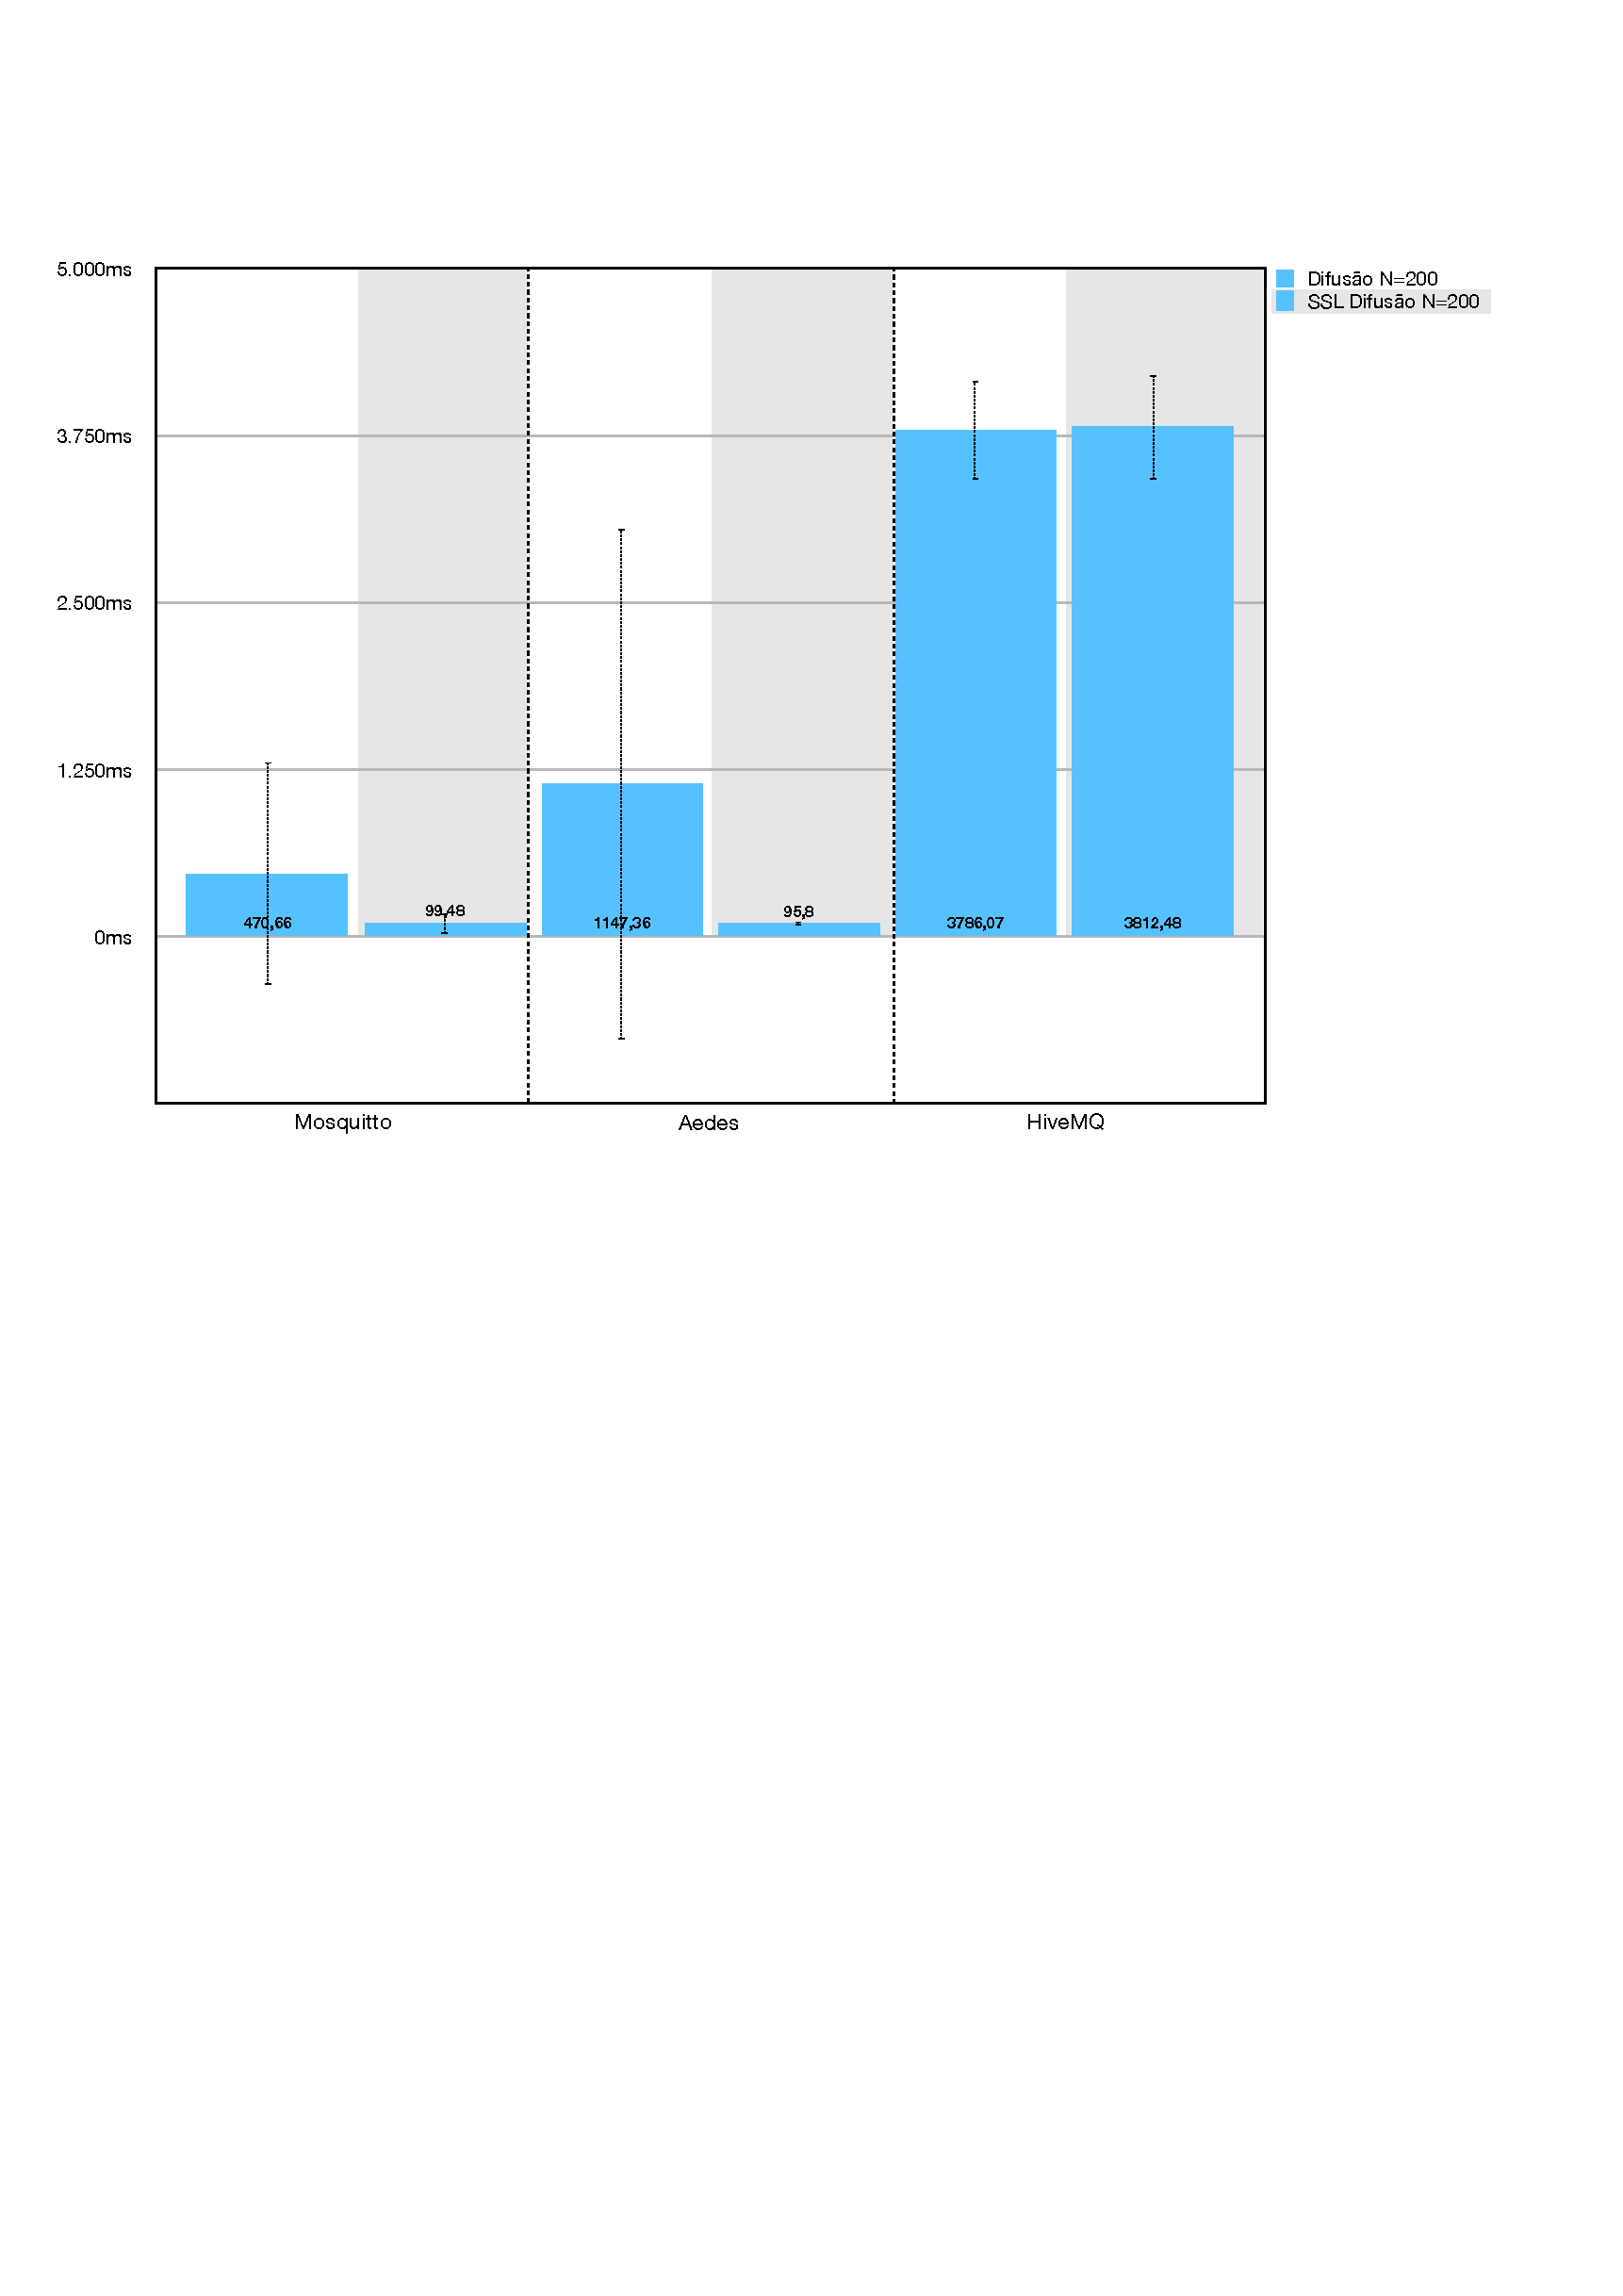
\includegraphics[width=1.0\textwidth]{local_spread2.pdf}
\end{center}
\subsection{Wi-Fi}
\subsubsection{Escrita/Leitura}
\begin{center}
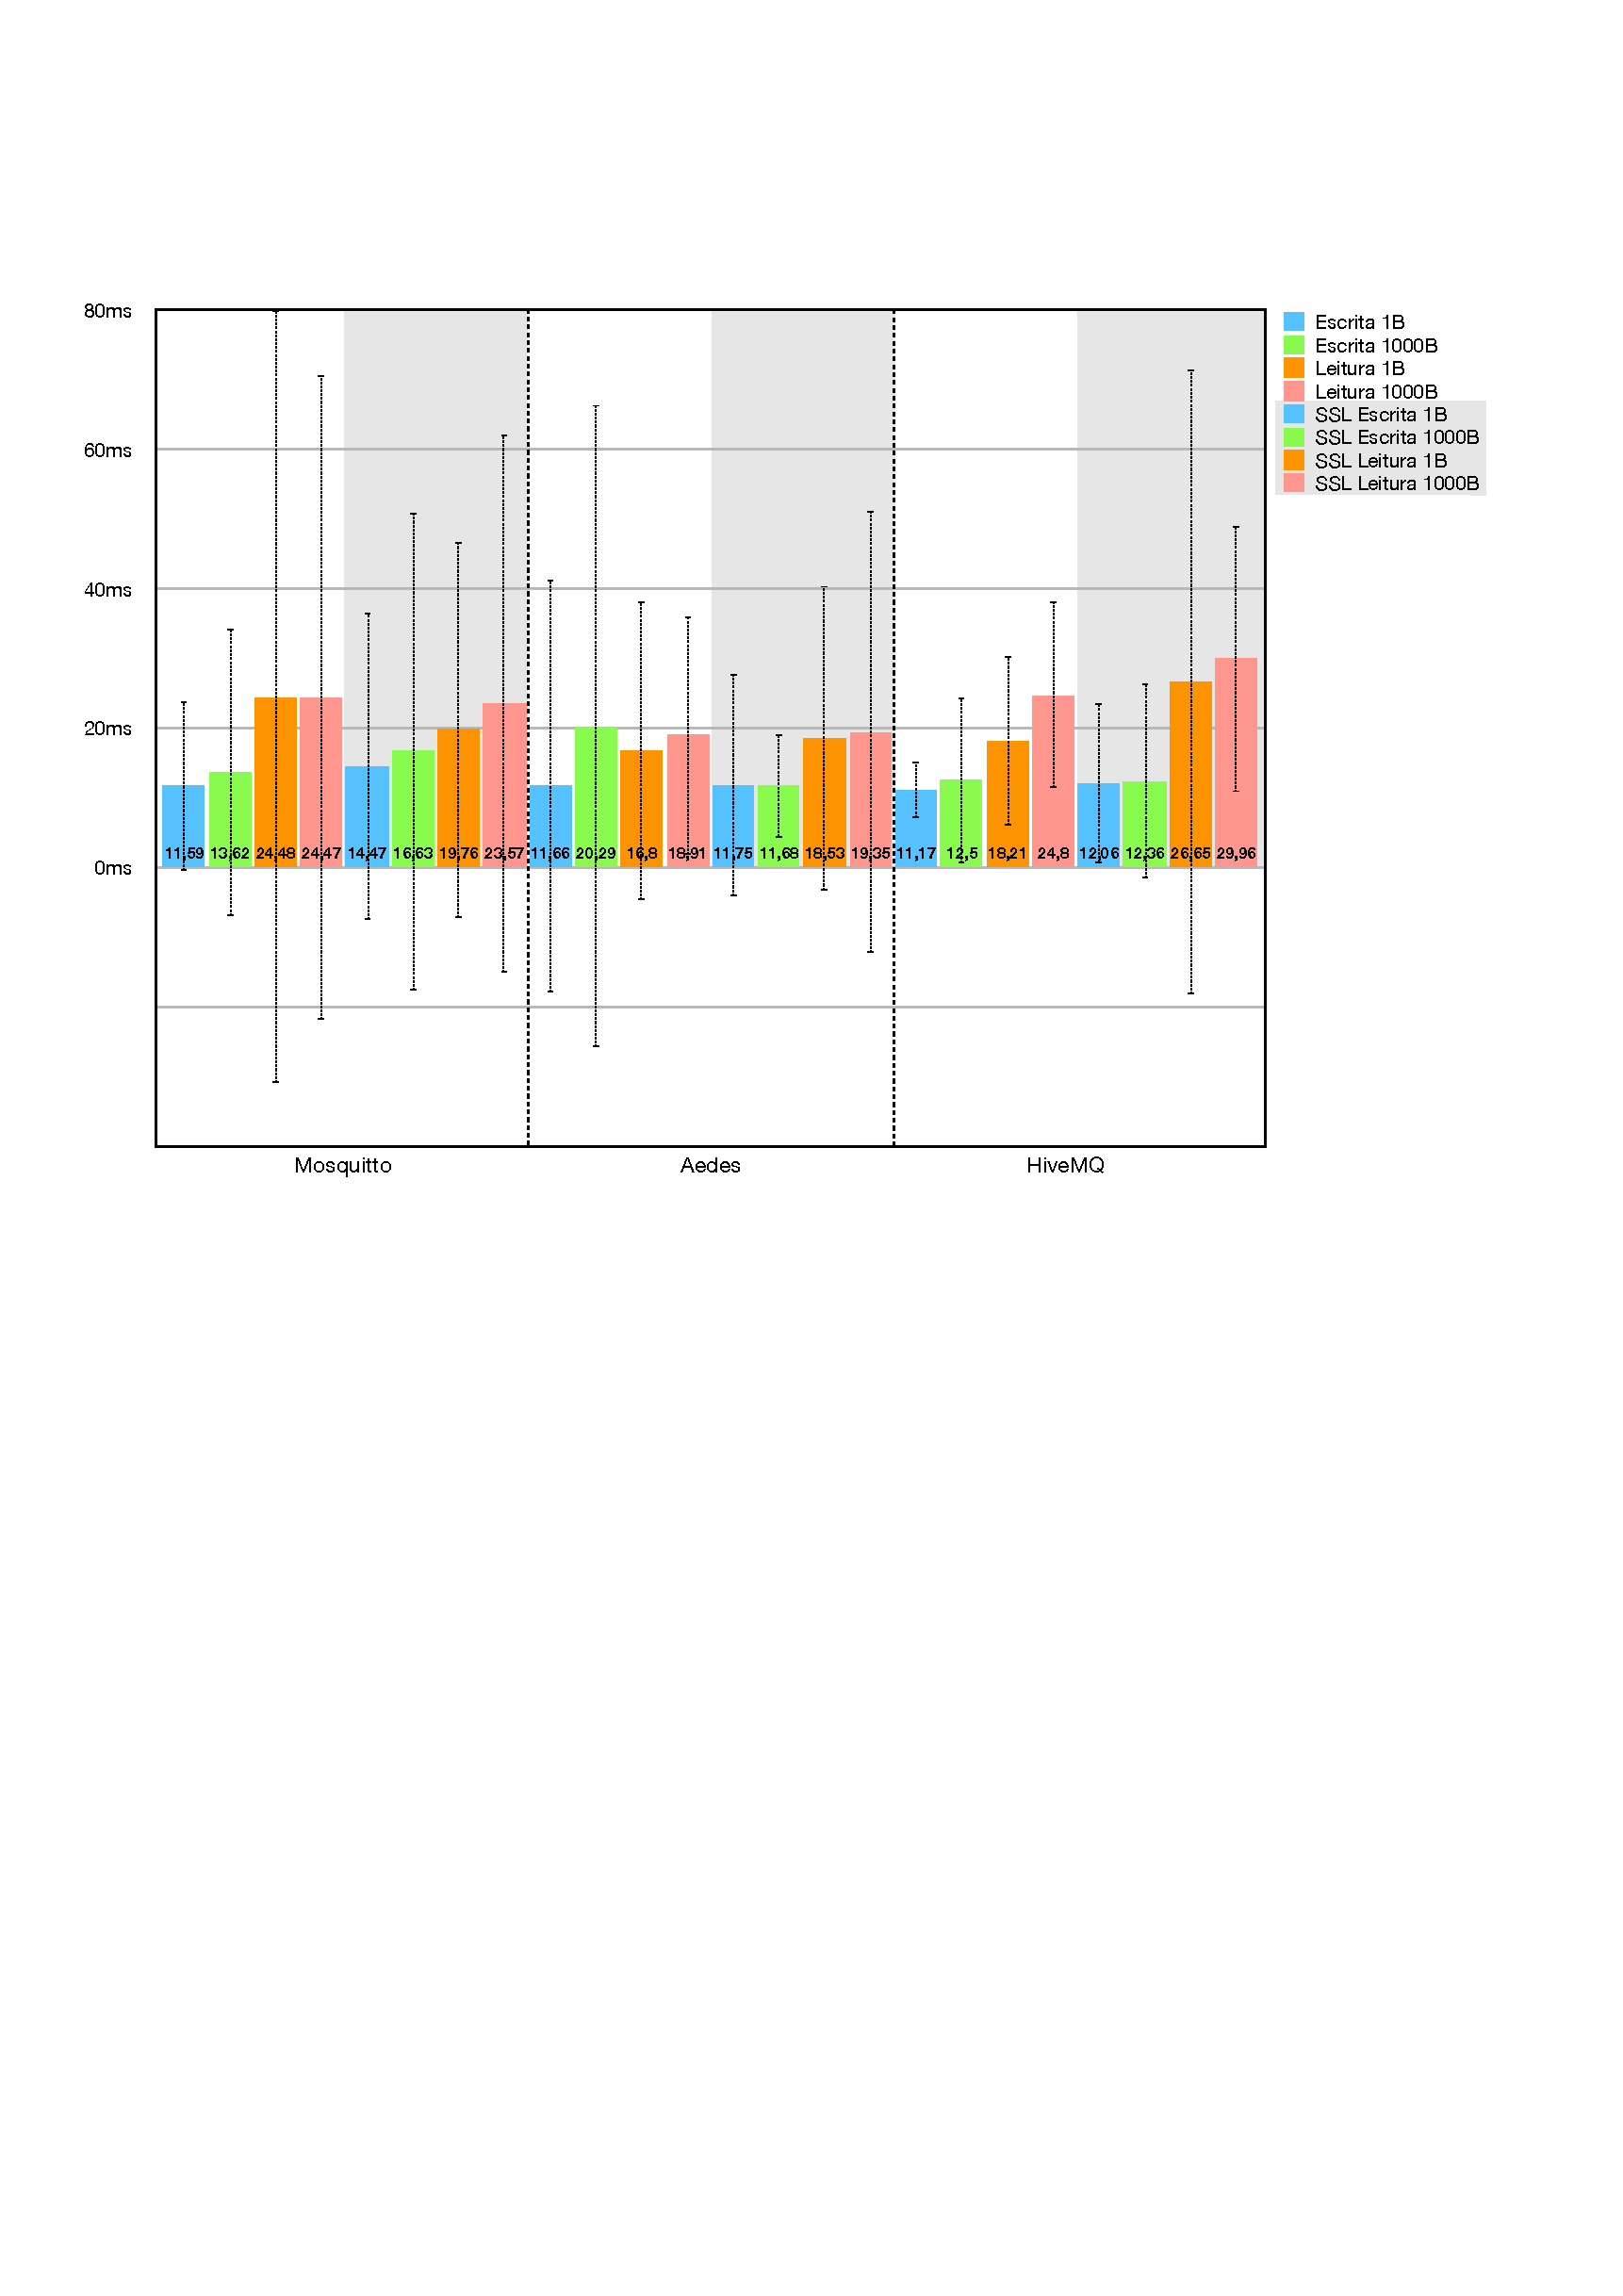
\includegraphics[width=1.0\textwidth]{wifi_wr.pdf}
\end{center}
\subsubsection{Difusão N = [10, 50, 100]}
\begin{center}
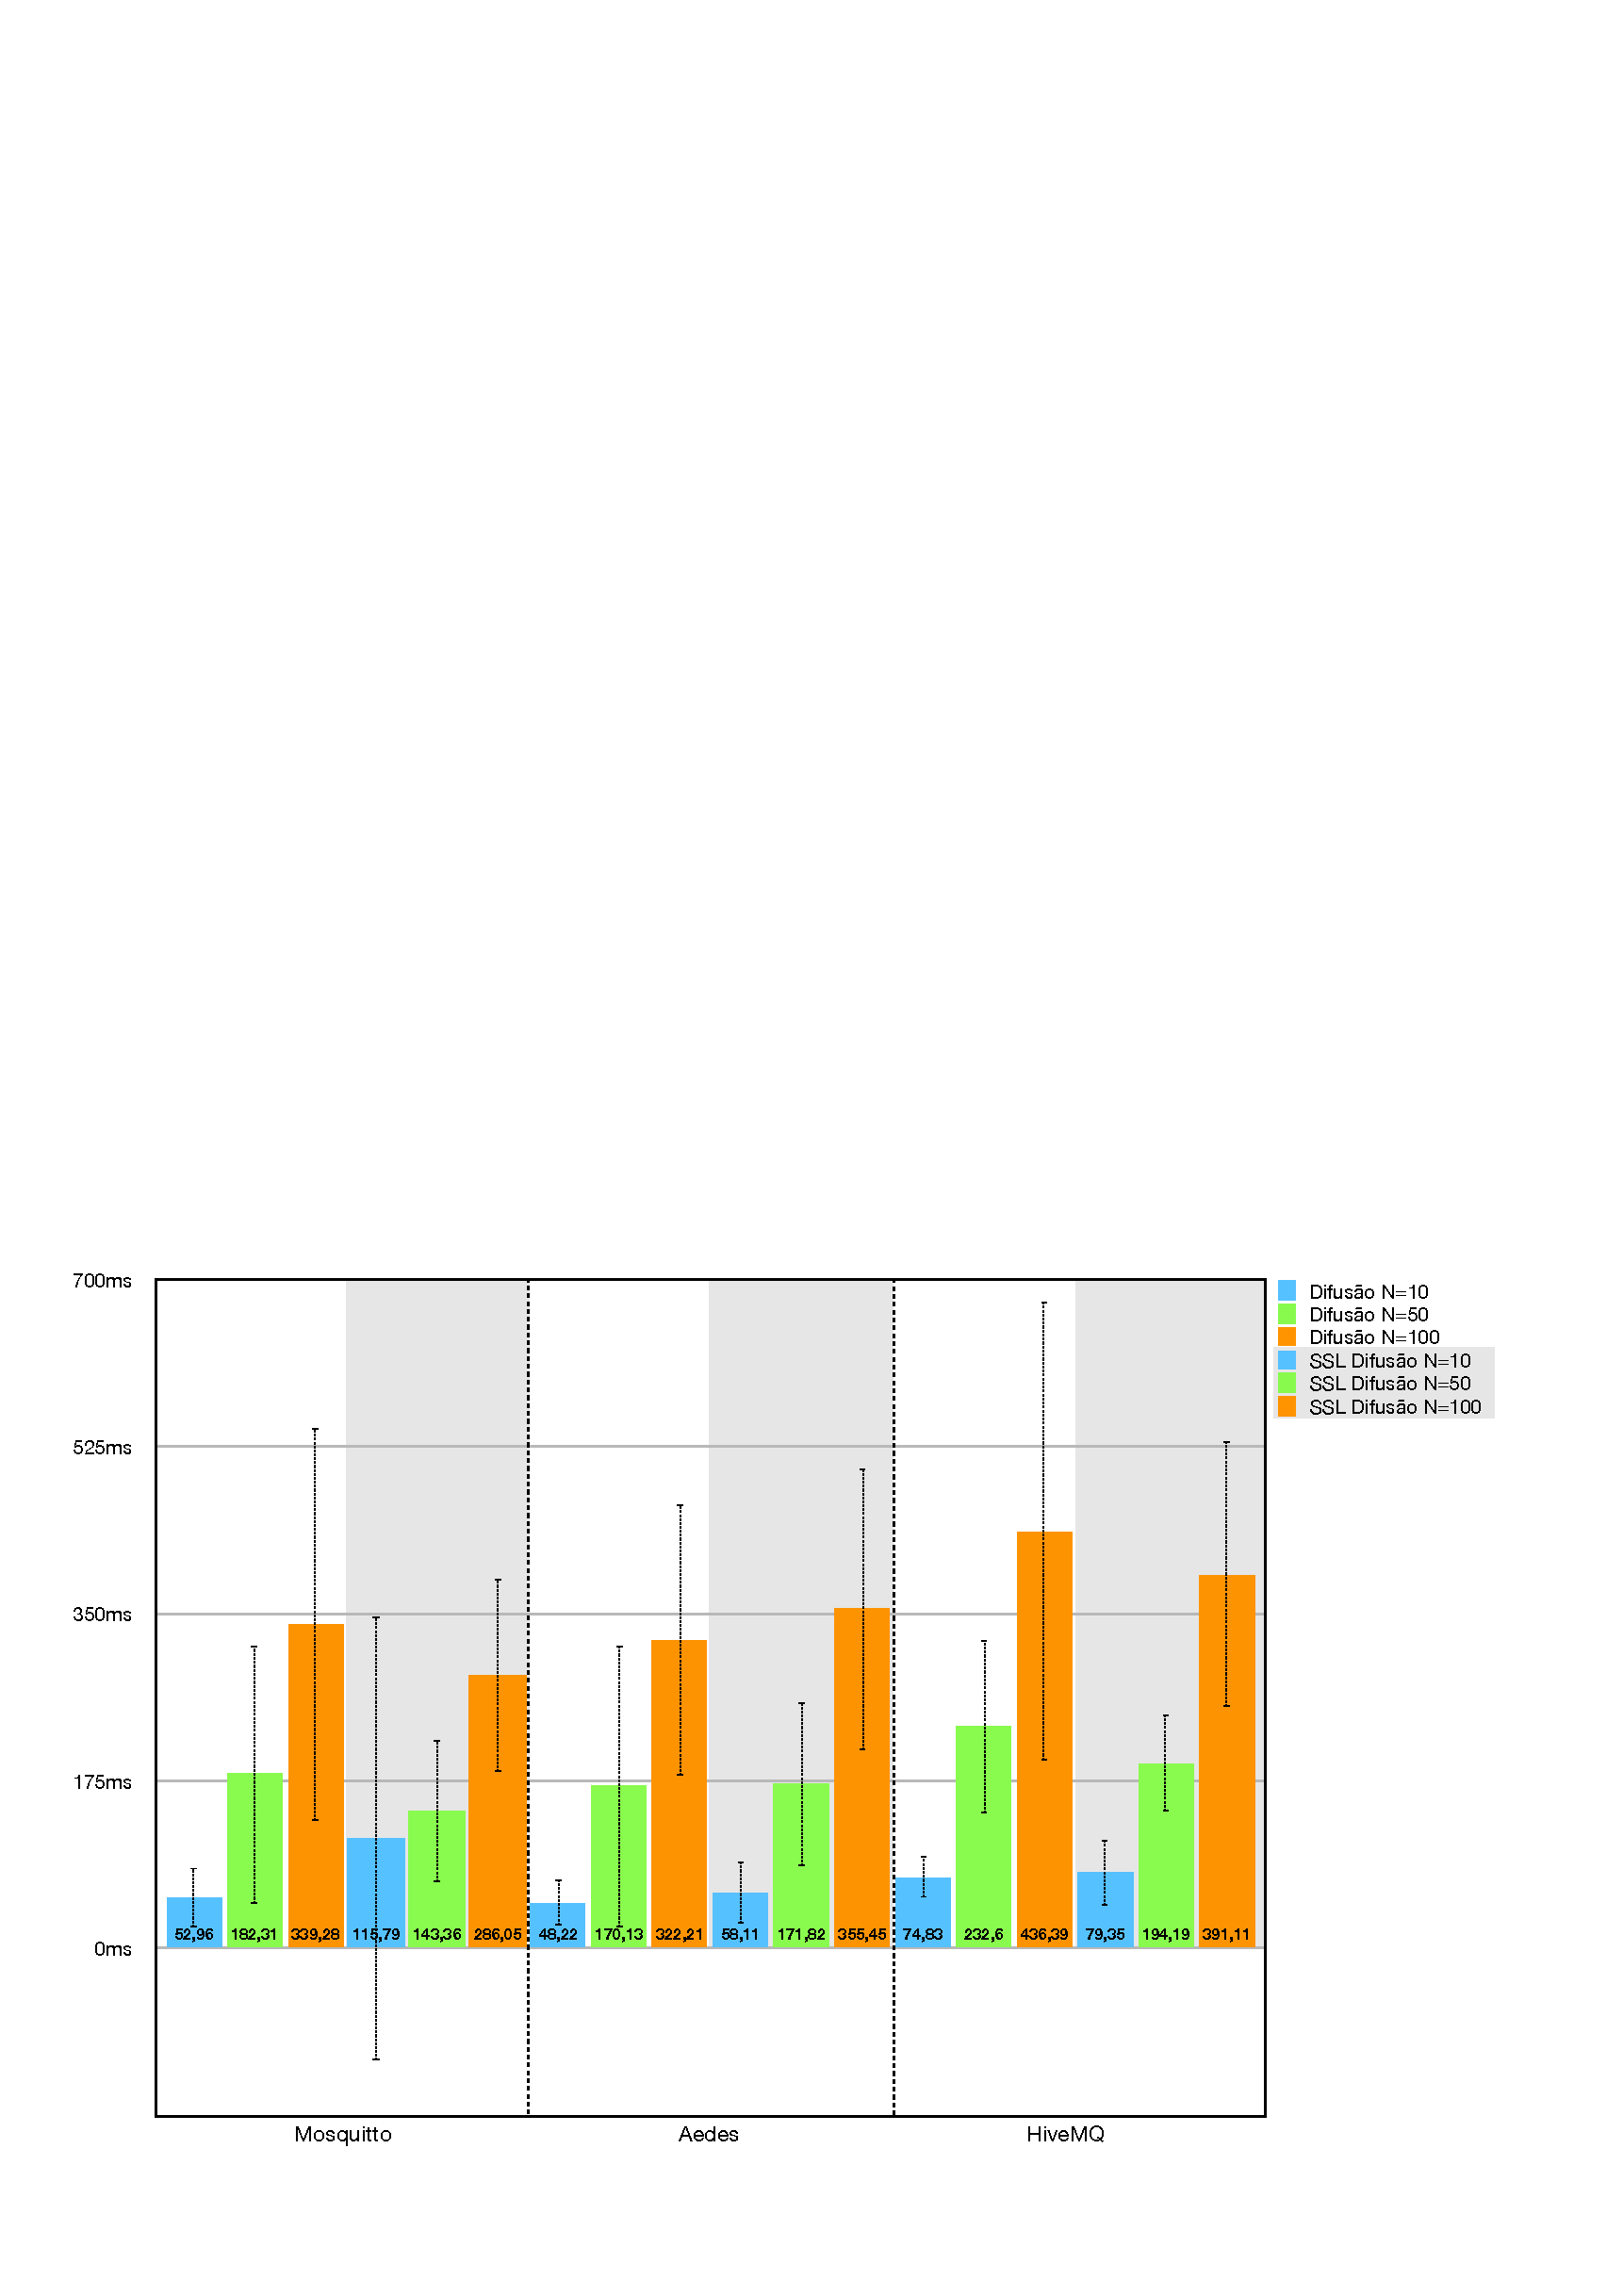
\includegraphics[width=1.0\textwidth]{wifi_spread1.pdf}
\end{center}
\subsubsection{Difusão N = 200}
\begin{center}
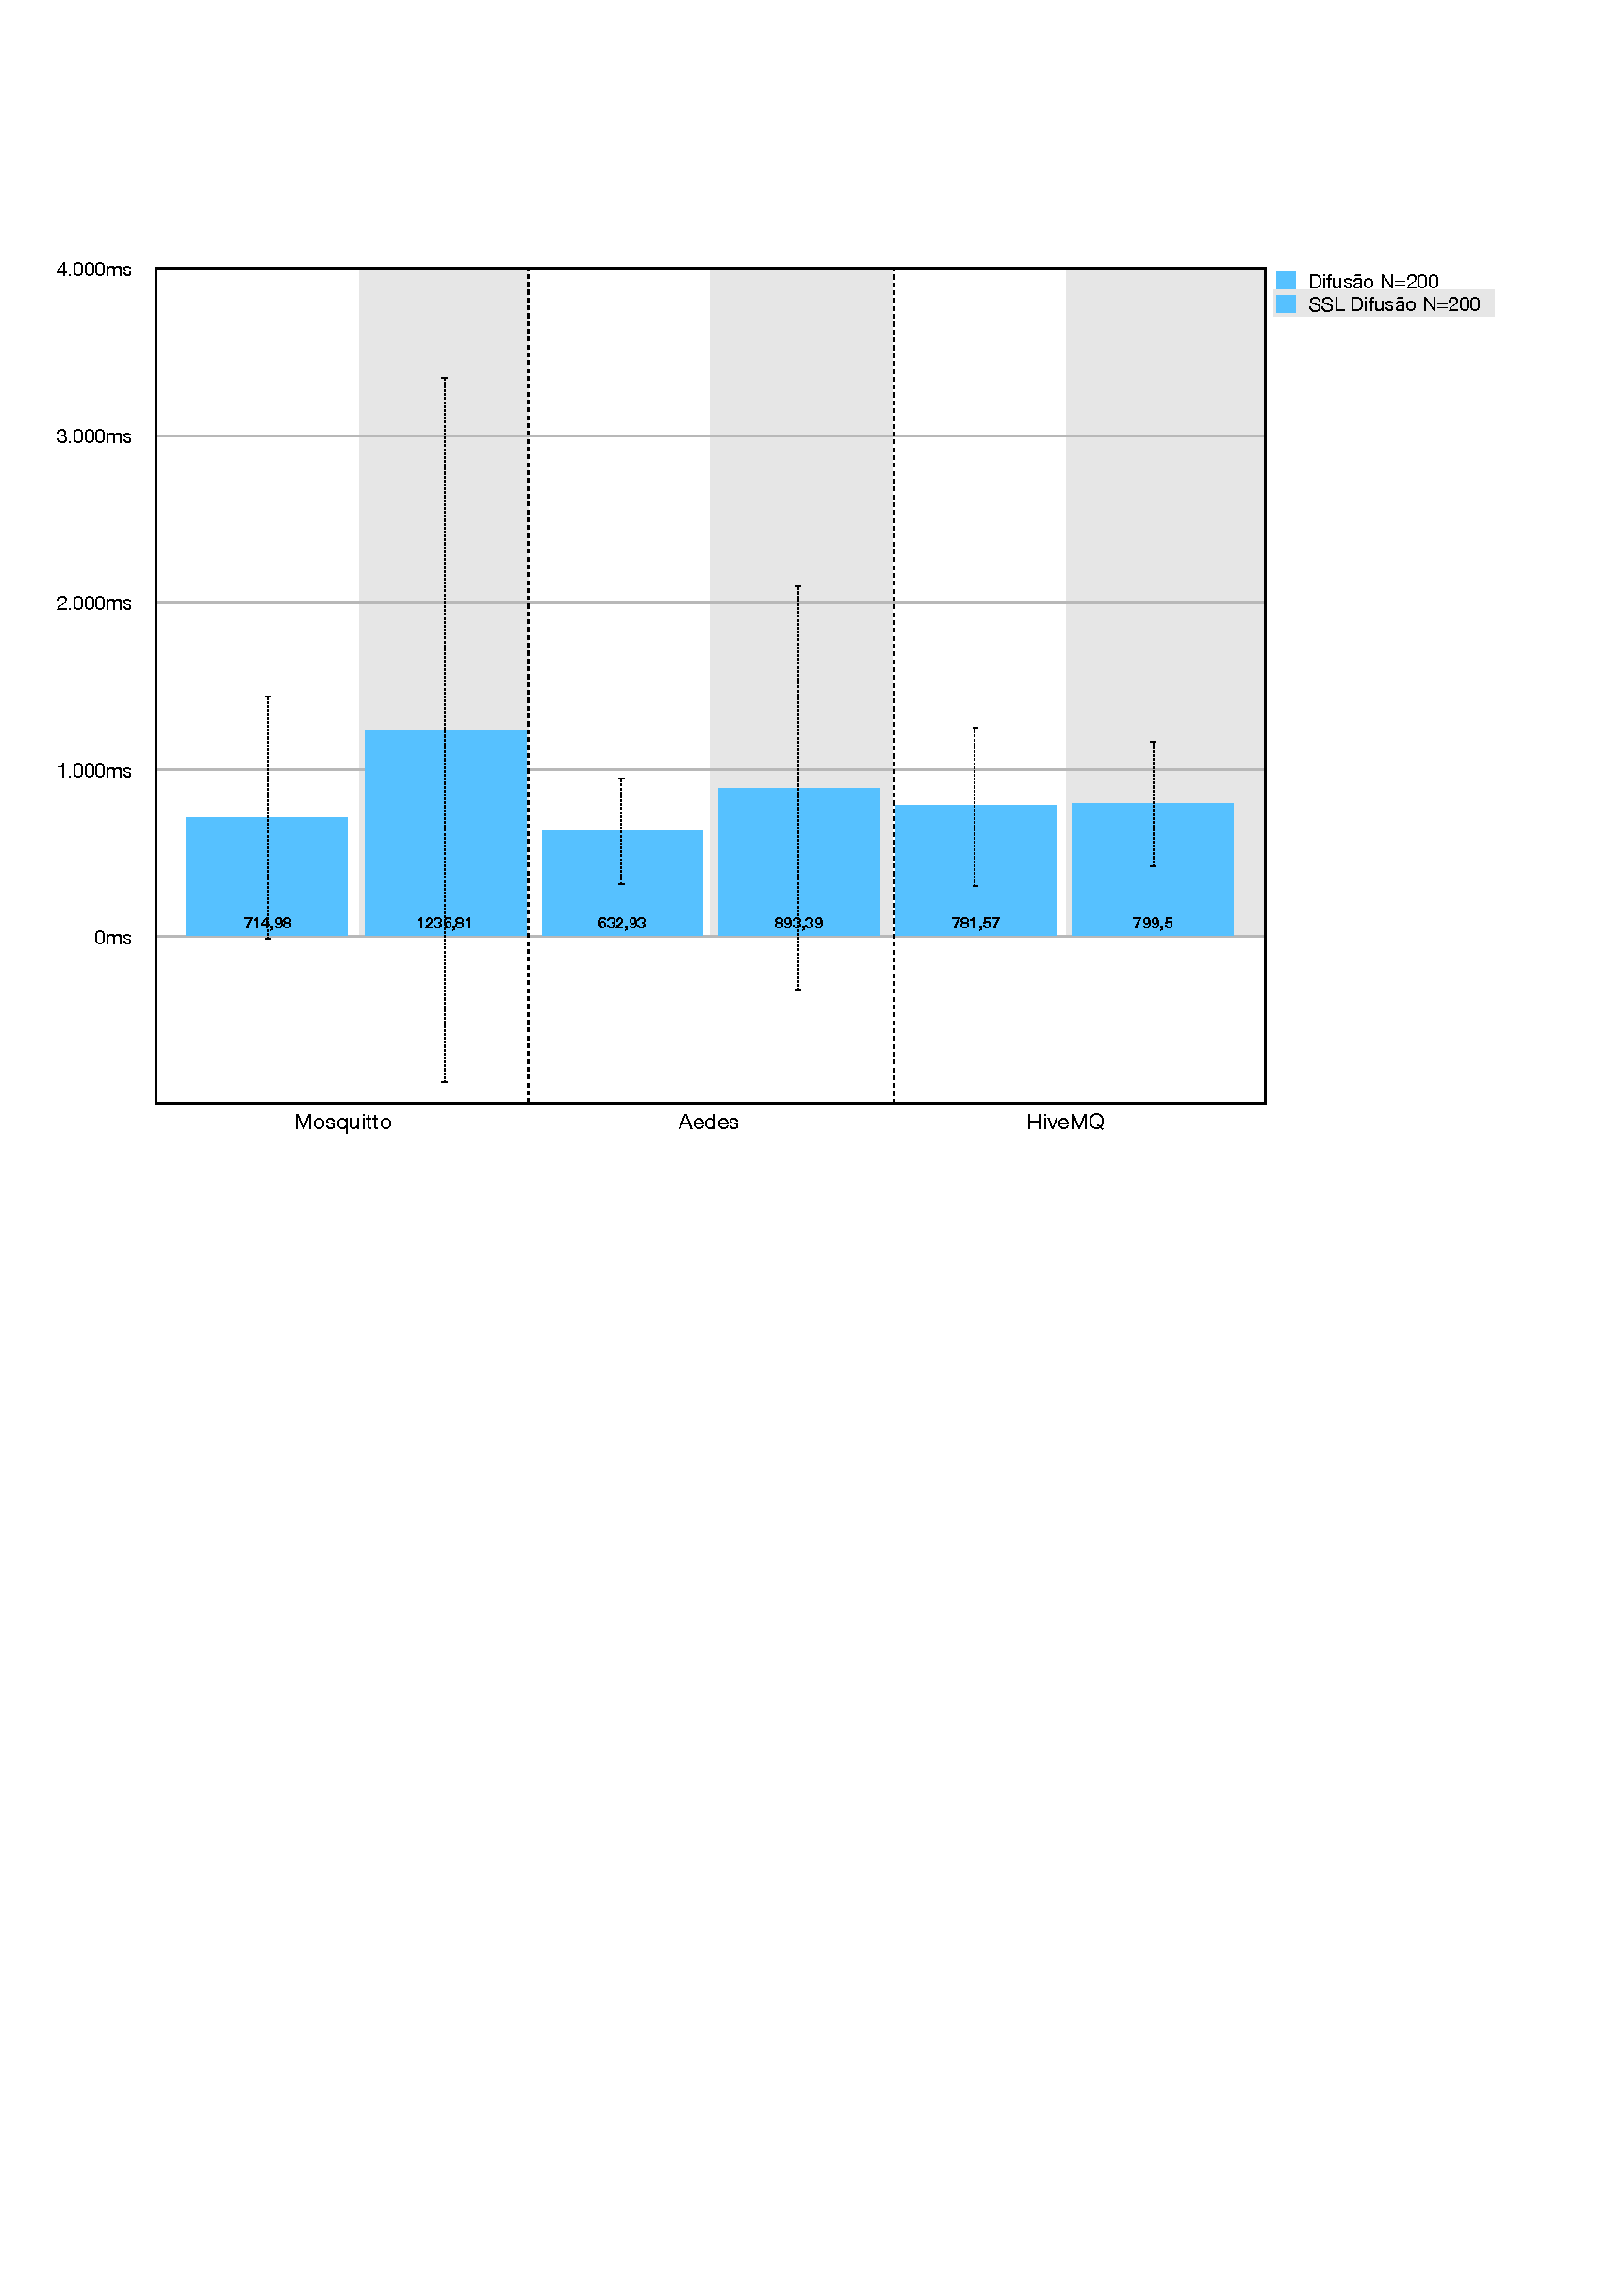
\includegraphics[width=1.0\textwidth]{wifi_spread2.pdf}
\end{center}
\subsection{Ethernet}
\subsubsection{Escrita/Leitura}
\begin{center}
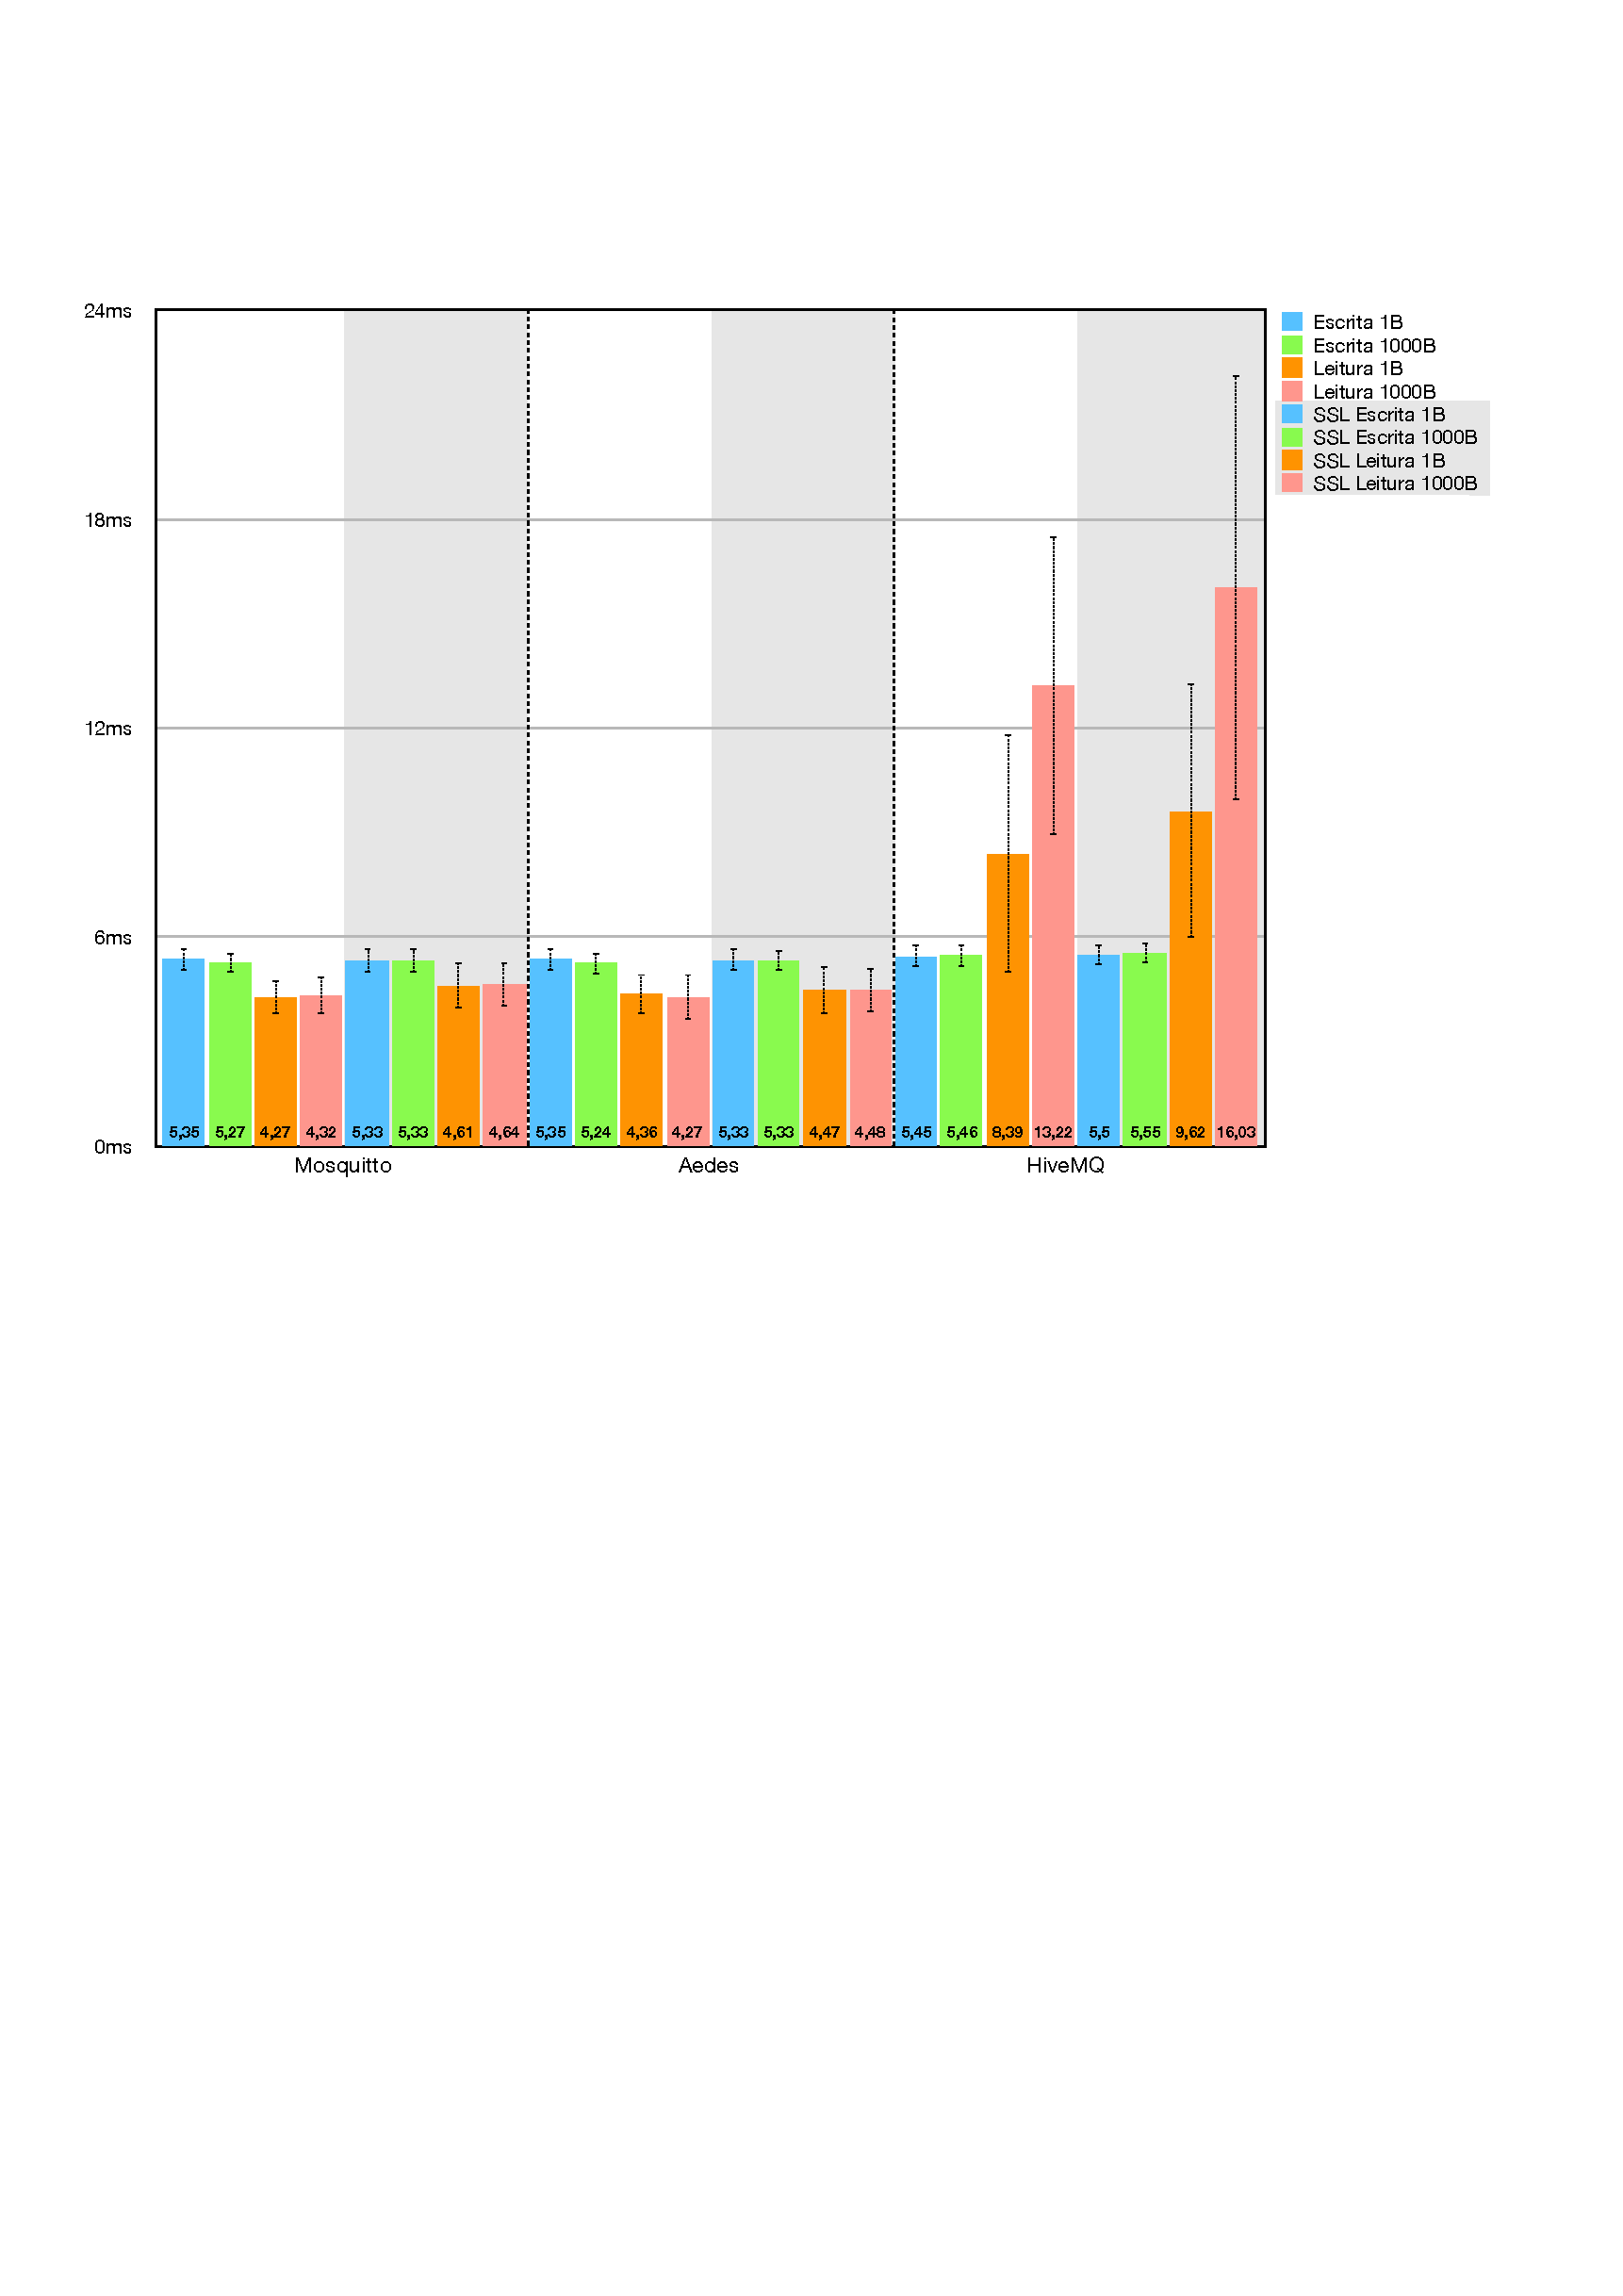
\includegraphics[width=1.0\textwidth]{eth_wr.pdf}
\end{center}
\subsubsection{Difusão N = [10, 50, 100]}
\begin{center}
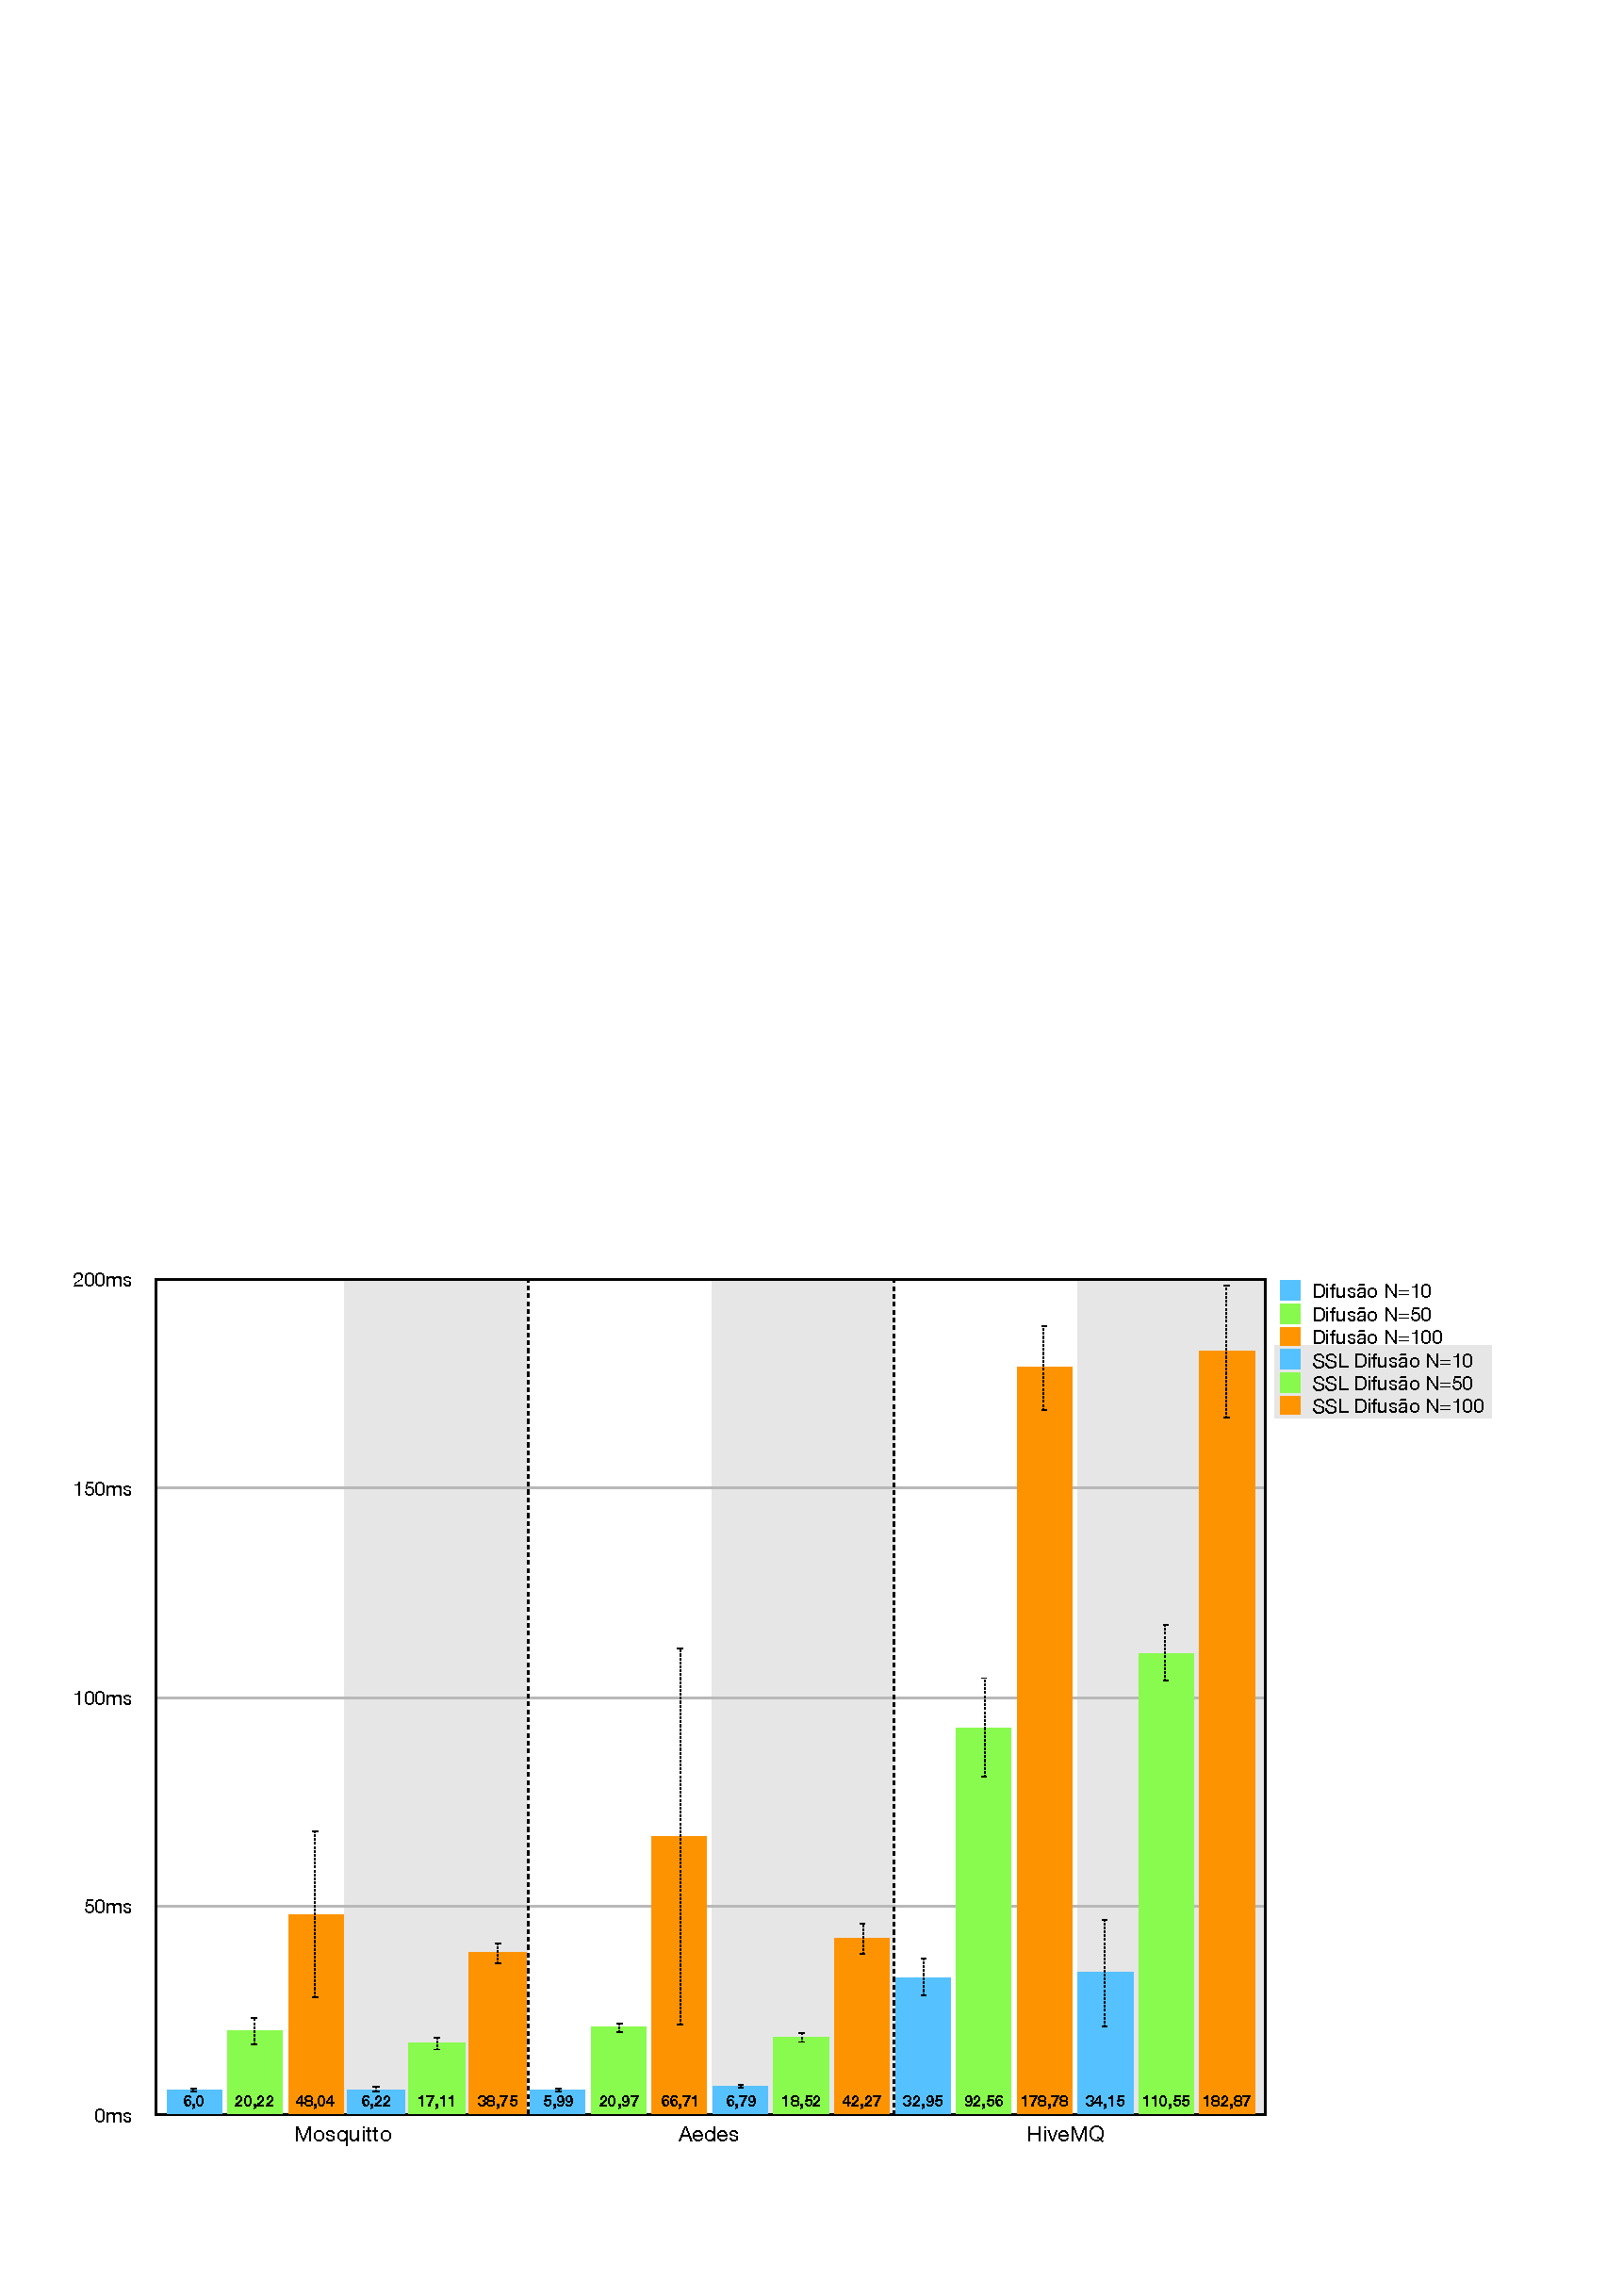
\includegraphics[width=1.0\textwidth]{eth_spread1.pdf}
\end{center}
\subsubsection{Difusão N = 200}
\begin{center}
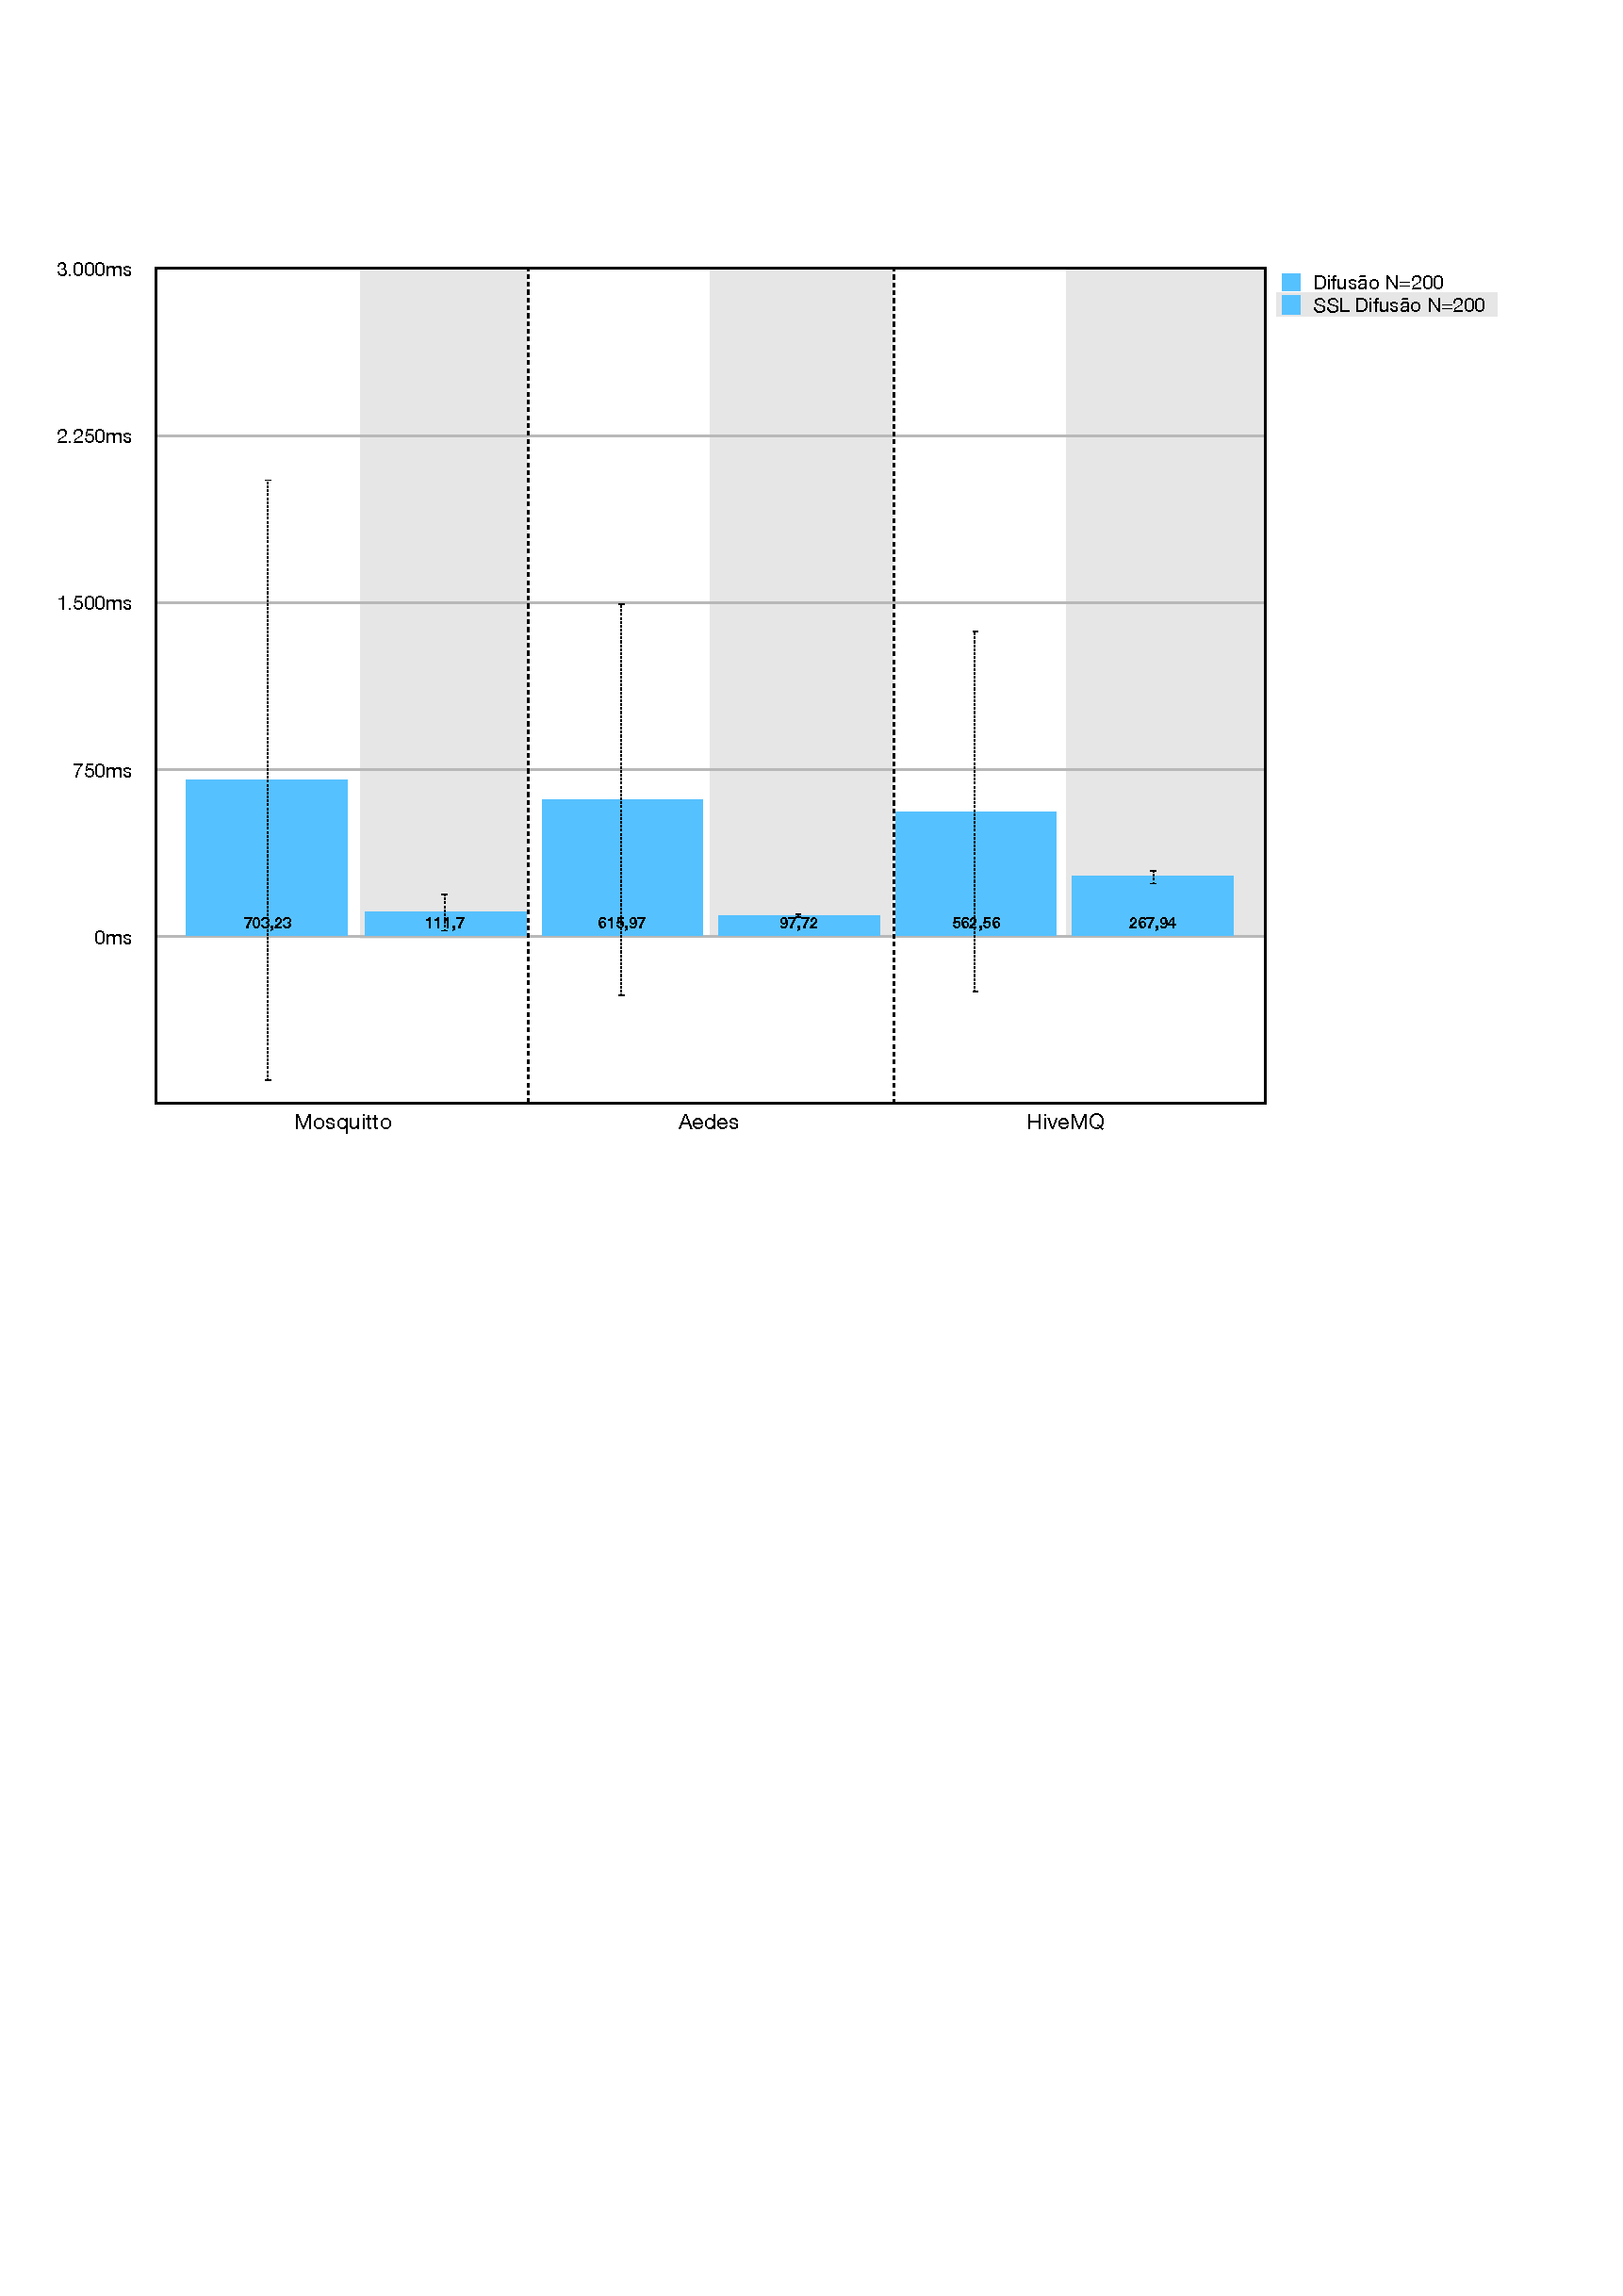
\includegraphics[width=1.0\textwidth]{eth_spread2.pdf}
\end{center}

\section{Conclusões}

As implementações \textit{Mosquitto} e \textit{Aedes} apresentaram desempenho muito semelhante em todos os testes. Além disso, nos testes de difusão, as duas apresentaram crescimento do tempo de resposta compatível com o crescimento do número de nós na rede. 

A implementação \textit{HiveMQ} apresentou desempenho significativamente mais lento do que as outras, por mais que tenha apresentado tempo de resposta até mais rápido em dois testes de difusão com $N = 200$. Também o desempenho extremamente lento na interface virtual de \textit{loopback} indica que pode haver algum \textit{bug} provocando inconsistência na resposta.

Recomendo a integração do servidor \textit{Mosquitto} à plataforma, devido ao bom desempenho e à estabilidade demonstrada.
    
\end{document}